%%%%%%%%%%%%%%%%%%%%%%%%%%%%% Thesis.tex %%%%%%%%%%%%%%%%%%%%%%%%%%%%%%%
%                                                                      %
%  ---------- Master of Science Dissertation template ----------       %
%                                                                      %
%  Template for the Master Thesis according to the regulations         %
%  published by the Academic Board (Direcção Académica) at IST.        %
%                                                                      %
%  For up-to-date guide, please refer to the official website          %
%  http://academica.tecnico.ulisboa.pt/alunos/dissertacao-de-mestrado/ %
%                                                                      %
%       Andre C. Marta                                                 %
%       Area Cientifica de Mecanica Aplicada e Aeroespacial            %
%       Departamento de Engenharia Mecanica                            %
%       Instituto Superior Tecnico                                     %
%       Av. Rovisco Pais                                               %
%       1049-001 Lisboa                                                %
%       Portugal                                                       %
%       Tel: +351 21 841 9469                                          %
%                        3469 (extension)                              %
%       Email: andre.marta@tecnico.ulisboa.pt                          %
%                                                                      %
%  Created:       Jan 20, 2011                                         %
%  Last Modified: Feb 19, 2018                                         %
%                                                                      %
%%%%%%%%%%%%%%%%%%%%%%%%%%%%%%%%%%%%%%%%%%%%%%%%%%%%%%%%%%%%%%%%%%%%%%%%
%  Revision history                                                    %
%  v1 - 2011/01/24 - original template                                 %
%  v2 - 2012/10/30 - new IST image and glossary support                %
%  v3 - 2013/12/10 - update according to 2012/13 official guide        %
%  v4 - 2014/02/28 - new default for bibliography style                %
%  v5 - 2014/05/07 - update according to 2013/14 official guide        %
%  v6 - 2015/07/02 - cover page format fixed,                          %
%                    contents page numbering fixed,                    %
%                    better language support,                          %
%                    enhanced examples of tables,                      %
%                    new option for appendix page numbering format,    %
%                    custom bibliography style                         %
%  v7 - 2018/02/19 - multiple citations compressed                     %
%%%%%%%%%%%%%%%%%%%%%%%%%%%%%%%%%%%%%%%%%%%%%%%%%%%%%%%%%%%%%%%%%%%%%%%%
%                                                                      %
% To generate the PDF file, type "make" at the terminal prompt.        %
%                                                                      %
% The IST template LaTeX package was created by the author             %
% and it can be downloaded from:                                       %
% https://fenix.ist.utl.pt/homepage/ist31052/                          %
%                                                                      %
% The external packages can be downloaded from                         %
% the Comprehensive TeX Archive Network at http://www.ctan.org/        %
%                                                                      %
% List of LaTex symbols:                                               %
% http://www.ctan.org/tex-archive/info/symbols/comprehensive/          %
%                                                                      %
% Help with LaTex can be found at                                      %
% http://www.giss.nasa.gov/tools/latex/ltx-2.html                      %
% http://en.wikibooks.org/wiki/LaTeX                                   %
%%%%%%%%%%%%%%%%%%%%%%%%%%%%%%%%%%%%%%%%%%%%%%%%%%%%%%%%%%%%%%%%%%%%%%%%

%%%%%%%%%%%%%%%%%%%%%%%%%%%%%%%%%%%%%%%%%%%%%%%%%%%%%%%%%%%%%%%%%%%%%%%%
%     Preamble                                                         %
%%%%%%%%%%%%%%%%%%%%%%%%%%%%%%%%%%%%%%%%%%%%%%%%%%%%%%%%%%%%%%%%%%%%%%%%

% ----------------------------------------------------------------------
%  Set the document class
% ----------------------------------------------------------------------
\documentclass[10pt,a4paper,twoside]{report}

% ----------------------------------------------------------------------
% Define external packages, language, margins, fonts and new commands
% ----------------------------------------------------------------------
%%%%%%%%%%%%%%%%%%%%%%%%%%%%%%%%%%%%%%%%%%%%%%%%%%%%%%%%%%%%%%%%%%%%%%%%
%                                                                      %
%     File: Thesis_Preamble.tex                                        %
%     Tex Master: Thesis.tex                                           %
%                                                                      %
%     Author: Gonçalo Santos                                           %
%     Last modified : 20 Oct 2018                                      %
%                                                                      %
%%%%%%%%%%%%%%%%%%%%%%%%%%%%%%%%%%%%%%%%%%%%%%%%%%%%%%%%%%%%%%%%%%%%%%%%

% ----------------------------------------------------------------------
% Define document language.
% ----------------------------------------------------------------------

% 'inputenc' package
%
% Accept different input encodings.
% http://www.ctan.org/tex-archive/macros/latex/base/
%
% > allows typing non-english text in LaTeX sources.
%
% ******************************* SELECT *******************************
%\usepackage[latin1]{inputenc} % <<<<< Windows
\usepackage[utf8]{inputenc}   % <<<<< Linux
% ******************************* SELECT *******************************


% 'babel' package
%
% Multilingual support for Plain TeX or LaTeX.
% http://www.ctan.org/tex-archive/macros/latex/required/babel/
%
% > sets the variable names according to the language selected
%
% ******************************* SELECT *******************************
%\usepackage[portuguese]{babel} % <<<<< Portuguese
\usepackage[english]{babel} % <<<<< English
% ******************************* SELECT *******************************


% List of LaTeX variable names: \abstractname, \appendixname, \bibname,
%   \chaptername, \contentsname, \listfigurename, \listtablename, ...
% http://www.tex.ac.uk/cgi-bin/texfaq2html?label=fixnam
%
% Changing the words babel uses (uncomment and redefine as necessary...)
%
\newcommand{\acknowledgments}{@undefined} % new LaTeX variable name
%
% > English
%
\addto\captionsenglish{\renewcommand{\acknowledgments}{Acknowledgments}}
%\addto\captionsenglish{\renewcommand{\listtablename}{List of Tables}}
%\addto\captionsenglish{\renewcommand{\listfigurename}{List of Figures}}
%\addto\captionsenglish{\renewcommand{\nomname}{Nomenclature}}
%\addto\captionsenglish{\renewcommand{\appendixname}{Appendix}}
%\addto\captionsenglish{\renewcommand{\bibname}{References}} % Bibliography

% > Portuguese
%
\addto\captionsportuguese{\renewcommand{\acknowledgments}{Agradecimentos}}
%\addto\captionsportuguese{\renewcommand{\listtablename}{Lista de Figuras}}
%\addto\captionsportuguese{\renewcommand{\listfigurename}{Lista de Tabelas}}
\addto\captionsportuguese{\renewcommand{\nomname}{Lista de S\'{i}mbolos}} % Nomenclatura
%\addto\captionsportuguese{\renewcommand{\appendixname}{Anexo}} % Apendice
%\addto\captionsportuguese{\renewcommand{\bibname}{Refer\^{e}ncias}} % Bibliografia


% ----------------------------------------------------------------------
% Define default and cover page fonts.
% ----------------------------------------------------------------------

% Use Arial font as default
%
\renewcommand{\rmdefault}{phv}
\renewcommand{\sfdefault}{phv}

% Define cover page fonts
%
%         encoding     family       series      shape
%  \usefont{T1}     {phv}=helvetica  {b}=bold    {n}=normal
%                   {ptm}=times      {m}=normal  {sl}=slanted
%                                                {it}=italic
% see more examples at
% http://julien.coron.free.fr/languages/latex/fonts/
%
\def\FontLn{% 16 pt normal
  \usefont{T1}{phv}{m}{n}\fontsize{16pt}{16pt}\selectfont}
\def\FontLb{% 16 pt bold
  \usefont{T1}{phv}{b}{n}\fontsize{16pt}{16pt}\selectfont}
\def\FontMn{% 14 pt normal
  \usefont{T1}{phv}{m}{n}\fontsize{14pt}{14pt}\selectfont}
\def\FontMb{% 14 pt bold
  \usefont{T1}{phv}{b}{n}\fontsize{14pt}{14pt}\selectfont}
\def\FontSn{% 12 pt normal
  \usefont{T1}{phv}{m}{n}\fontsize{12pt}{12pt}\selectfont}


% ----------------------------------------------------------------------
% Define page margins and line spacing.
% ----------------------------------------------------------------------

% 'geometry' package
%
% Flexible and complete interface to document dimensions.
% http://www.ctan.org/tex-archive/macros/latex/contrib/geometry/
%
% > set the page margins (2.5cm minimum in every side, as per IST rules)
%
\usepackage{geometry}	
\geometry{verbose,tmargin=2.5cm,bmargin=2.5cm,lmargin=2.5cm,rmargin=2.5cm}

% 'setspace' package
%
% Set space between lines.
% http://www.ctan.org/tex-archive/macros/latex/contrib/setspace/
%
% > allow setting line spacing (line spacing of 1.5, as per IST rules)
%
\usepackage{setspace}
\renewcommand{\baselinestretch}{1.5}


% ----------------------------------------------------------------------
% Include external packages.
% Note that not all of these packages may be available on all system
% installations. If necessary, include the .sty files locally in
% the <jobname>.tex file directory.
% ----------------------------------------------------------------------

% 'graphicx' package
%
% Enhanced support for graphics.
% http://www.ctan.org/tex-archive/macros/latex/required/graphics/
%
% > extends arguments of the \includegraphics command
%
\usepackage{graphicx}


% 'color' package
%
% Colour control for LaTeX documents.
% http://www.ctan.org/tex-archive/macros/latex/required/graphics/
%
% > defines color macros: \color{<color name>}
%
%\usepackage{color}


% 'amsmath' package
%
% Mathematical enhancements for LaTeX.
% http://www.ctan.org/tex-archive/macros/latex/required/amslatex/
%
% > American Mathematical Society plain Tex macros
%
\usepackage{amsmath}  % AMS mathematical facilities for LaTeX.
\usepackage{amsthm}   % Typesetting theorems (AMS style).
\usepackage{amsfonts} %


% 'wrapfig' package
%
% Produces figures which text can flow around.
% http://www.ctan.org/tex-archive/macros/latex/contrib/wrapfig/
%
% > wrap figures/tables in text (i.e., Di Vinci style)
%
% \usepackage{wrapfig}


% 'subfigure' package
%
% Deprecated: Figures divided into subfigures.
% http://www.ctan.org/tex-archive/obsolete/macros/latex/contrib/subfigure/
%
% > subcaptions for subfigures
%
\usepackage{subfigure}


% 'subfigmat' package
%
% Automates layout when using the subfigure package.
% http://www.ctan.org/tex-archive/macros/latex/contrib/subfigmat/
%
% > matrices of similar subfigures
%
\usepackage{subfigmat}


% 'url' package
%
% Verbatim with URL-sensitive line breaks.
% http://www.ctan.org/tex-archive/macros/latex/contrib/url/
%
% > URLs in BibTex
%
% \usepackage{url}


% 'varioref' package
%
% Intelligent page references.
% http://www.ctan.org/tex-archive/macros/latex/required/tools/
%
% > smart page, figure, table and equation referencing
%
%\usepackage{varioref}


% 'dcolumn' package
%
% Align on the decimal point of numbers in tabular columns.
% http://www.ctan.org/tex-archive/macros/latex/required/tools/
%
% > decimal-aligned tabular math columns
%
\usepackage{dcolumn}
\newcolumntype{d}{D{.}{.}{-1}} % column aligned by the point separator '.'
\newcolumntype{e}{D{E}{E}{-1}} % column aligned by the exponent 'E'


% '' package
%
% Reimplementation of and extensions to LaTeX verbatim.
% http://www.ctan.org/tex-archive/macros/latex/required/tools/
%
% > provides the verbatim environment (\begin{verbatim},\end{verbatim})
%   and a comment environment (\begin{comment},  \end{comment})
%
% \usepackage{verbatim}


% 'moreverb' package
%
% Extended verbatim.
% http://www.ctan.org/tex-archive/macros/latex/contrib/moreverb/
%
% > supports tab expansion and line numbering
%
% \usepackage{moreverb}



% 'nomencl' package
%
% Produce lists of symbols as in nomenclature.
% http://www.ctan.org/tex-archive/macros/latex/contrib/nomencl/
%
% The nomencl package makes use of the MakeIndex program
% in order to produce the nomenclature list.
%
% Nomenclature
% 1: On running the file through LATEX, the command \makenomenclature
%    in the preamble instructs it to create/open the nomenclature file
%    <jobname>.nlo corresponding to the LATEX file <jobname>.tex and
%    writes the information from the \nomenclature commands to this file.
% 2: The next step is to invoke MakeIndex in order to produce the
%    <jobname>.nls file. This can be achieved by making use of the
%    command: makeindex <jobname>.nlo -s nomencl.ist -o <jobname>.nls
% 3: The last step is to invoke LATEX on the <jobname>.tex file once
%    more. There, the \printnomenclature in the document will input the
%    <jobname>.nls file and process it according to the given options.
%
% http://www-h.eng.cam.ac.uk/help/tpl/textprocessing/nomencl.pdf
%
% Nomenclature (produces *.nlo *.nls files)
\usepackage{nomencl}
\makenomenclature
%
% Group variables according to their symbol type
%
\RequirePackage{ifthen}
\ifthenelse{\equal{\languagename}{english}}%
    { % English
    \renewcommand{\nomgroup}[1]{%
      \ifthenelse{\equal{#1}{R}}{%
        \item[\textbf{Roman symbols}]}{%
        \ifthenelse{\equal{#1}{G}}{%
          \item[\textbf{Greek symbols}]}{%
          \ifthenelse{\equal{#1}{S}}{%
            \item[\textbf{Subscripts}]}{%
            \ifthenelse{\equal{#1}{T}}{%
              \item[\textbf{Superscripts}]}{}}}}}%
    }{% Portuguese
    \renewcommand{\nomgroup}[1]{%
      \ifthenelse{\equal{#1}{R}}{%
        \item[\textbf{Simbolos romanos}]}{%
        \ifthenelse{\equal{#1}{G}}{%
          \item[\textbf{Simbolos gregos}]}{%
          \ifthenelse{\equal{#1}{S}}{%
            \item[\textbf{Subscritos}]}{%
            \ifthenelse{\equal{#1}{T}}{%
              \item[\textbf{Sobrescritos}]}{}}}}}%
    }%


% 'glossary' package
%
% Create a glossary.
% http://www.ctan.org/tex-archive/macros/latex/contrib/glossary/
%
% Glossary (produces *.glo *.ist files)
\usepackage[number=none]{glossary}
% (remove blank line between groups)
\setglossary{gloskip={}}
% (redefine glossary style file)
%\renewcommand{\istfilename}{myGlossaryStyle.ist}
\makeglossary


% 'rotating' package
%
% Rotation tools, including rotated full-page floats.
% http://www.ctan.org/tex-archive/macros/latex/contrib/rotating/
%
% > show wide figures and tables in landscape format:
%   use \begin{sidewaystable} and \begin{sidewaysfigure}
%   instead of 'table' and 'figure', respectively.
%
\usepackage{rotating}


% 'hyperref' package
%
% Extensive support for hypertext in LaTeX.
% http://www.ctan.org/tex-archive/macros/latex/contrib/hyperref/
%
% > Extends the functionality of all the LATEX cross-referencing
%   commands (including the table of contents, bibliographies etc) to
%   produce \special commands which a driver can turn into hypertext
%   links; Also provides new commands to allow the user to write adhoc
%   hypertext links, including those to external documents and URLs.
%
\usepackage[pdftex]{hyperref} % enhance documents that are to be
                              % output as HTML and PDF
\hypersetup{colorlinks,       % color text of links and anchors,
                              % eliminates borders around links
%            linkcolor=red,    % color for normal internal links
            linkcolor=black,  % color for normal internal links
            anchorcolor=black,% color for anchor text
%            citecolor=green,  % color for bibliographical citations
            citecolor=black,  % color for bibliographical citations
%            filecolor=magenta,% color for URLs which open local files
            filecolor=black,  % color for URLs which open local files
%            menucolor=red,    % color for Acrobat menu items
            menucolor=black,  % color for Acrobat menu items
%            pagecolor=red,    % color for links to other pages
            pagecolor=black,  % color for links to other pages
%            urlcolor=cyan,    % color for linked URLs
            urlcolor=black,   % color for linked URLs
	          bookmarks=true,         % create PDF bookmarks
	          bookmarksopen=false,    % don't expand bookmarks
	          bookmarksnumbered=true, % number bookmarks
	          pdftitle={Thesis},
            pdfauthor={Andre C. Marta},
            pdfsubject={Thesis Title},
            pdfkeywords={Thesis Keywords},
            pdfstartview=FitV,
            pdfdisplaydoctitle=true}


% 'hypcap' package
%
% Adjusting the anchors of captions.
% http://www.ctan.org/tex-archive/macros/latex/contrib/oberdiek/
%
% > fixes the problem with hyperref, that links to floats points
%   below the caption and not at the beginning of the float.
%
\usepackage[figure,table]{hypcap}


% 'natbib' package
%
% Flexible bibliography support.
% http://www.ctan.org/tex-archive/macros/latex/contrib/natbib/
%
% > produce author-year style citations
%
% \citet  and \citep  for textual and parenthetical citations, respectively
% \citet* and \citep* that print the full author list, and not just the abbreviated one
% \citealt is the same as \citet but without parentheses. Similarly, \citealp is \citep without parentheses
% \citeauthor
% \citeyear
% \citeyearpar
%
\usepackage{natbib}


% ----------------------------------------------------------------------
% Define new commands to assure consistent treatment throughout document
% ----------------------------------------------------------------------

\newcommand{\ud}{\mathrm{d}}                % total derivative
\newcommand{\degree}{\ensuremath{^\circ\,}} % degrees

% Abbreviations

\newcommand{\mcol}{\multicolumn}            % table format

\newcommand{\eqnref}[1]{(\ref{#1})}
\newcommand{\class}[1]{\texttt{#1}}
\newcommand{\package}[1]{\texttt{#1}}
\newcommand{\file}[1]{\texttt{#1}}
\newcommand{\BibTeX}{\textsc{Bib}\TeX}

% Typefaces ( example: {\bf Bold text here} )
%
% > pre-defined
%   \bf % bold face
%   \it % italic
%   \tt % typewriter
%
% > newly defined
\newcommand{\tr}[1]{{\ensuremath{\textrm{#1}}}}   % text roman
\newcommand{\tb}[1]{{\ensuremath{\textbf{#1}}}}   % text bold face
\newcommand{\ti}[1]{{\ensuremath{\textit{#1}}}}   % text italic
\newcommand{\mc}[1]{{\ensuremath{\mathcal{#1}}}}  % math calygraphy
\newcommand{\mco}[1]{{\ensuremath{\mathcalold{#1}}}}% math old calygraphy
\newcommand{\mr}[1]{{\ensuremath{\mathrm{#1}}}}   % math roman
\newcommand{\mb}[1]{{\ensuremath{\mathbf{#1}}}}   % math bold face
\newcommand{\bs}[1]{\ensuremath{\boldsymbol{#1}}} % math symbol
\def\bm#1{\mathchoice                             % math bold
  {\mbox{\boldmath$\displaystyle#1$}}%
  {\mbox{\boldmath$#1$}}%
  {\mbox{\boldmath$\scriptstyle#1$}}%
  {\mbox{\boldmath$\scriptscriptstyle#1$}}}
\newcommand{\boldcal}[1]{{\ensuremath{\boldsymbol{\mathcal{#1}}}}}% math bold calygraphy

\usepackage{fancyvrb}
 % file "Thesis_Preamble.tex"

%%%%%%%%%%%%%%%%%%%%%%%%%%%%%%%%%%%%%%%%%%%%%%%%%%%%%%%%%%%%%%%%%%%%%%%%
%     Begin Document                                                   %
%%%%%%%%%%%%%%%%%%%%%%%%%%%%%%%%%%%%%%%%%%%%%%%%%%%%%%%%%%%%%%%%%%%%%%%%
\begin{document}

% Set plain page style (no headers, footer with centered page number)
\pagestyle{plain}

% Set roman numbering (i,ii,...) before the start of chapters
\pagenumbering{roman}

% ----------------------------------------------------------------------
%  Cover page
% ----------------------------------------------------------------------
%%%%%%%%%%%%%%%%%%%%%%%%%%%%%%%%%%%%%%%%%%%%%%%%%%%%%%%%%%%%%%%%%%%%%%%%
%                                                                      %
%     File: Thesis_FrontCover.tex                                      %
%     Tex Master: Thesis.tex                                           %
%                                                                      %
%     Author: Gonçalo Santos                                           %
%     Last modified : 20 Oct 2018                                      %
%                                                                      %
%%%%%%%%%%%%%%%%%%%%%%%%%%%%%%%%%%%%%%%%%%%%%%%%%%%%%%%%%%%%%%%%%%%%%%%%

\thispagestyle {empty}

% IST Logo
% parameters: bb=llx lly urx ury (bounding box), width=h_length, height=v_length, angle=angle, scale=factor, clip=true/false, draft=true/false.
\vspace*{-12mm}
\hspace*{-12mm}

\includegraphics[height=20mm]{IST_A_CMYK_POS-crop.pdf}

\begin{center}
%
% Figure (Image or plot)
\vspace{0.5cm}
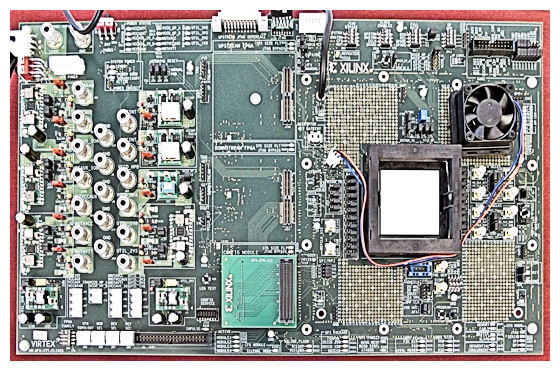
\includegraphics[height=60mm]{Figures/fpga.jpg}

% Title, author and degree
\vspace{0.8cm}
{\FontLb C Compiler for the VERSAT Reconfigurable Processor} \\
\vspace{3.6cm}
{\FontMb Gonçalo da Conceição Reis dos Santos} \\
\vspace{1.9cm}
{\FontLn Thesis to obtain the Master of Science Degree in} \\
\vspace{0.3cm}
{\FontLb Electrical and Computer Engineering} \\
%\vspace{1.9cm}
\vspace{1.0cm}
{\FontSn %
\begin{tabular}{ll}
Supervisor: & Prof. José João Henriques Teixeira de Sousa
\end{tabular} } \\
\vspace{1.0cm}
{\FontMb Examination Committee} \\
\vspace{0.3cm}
{\FontSn %
\begin{tabular}{ll}
Chairperson: & Prof. Francisco André Corrêa Alegria\\
Supervisor: & Prof. José João Henriques Teixeira de Sousa \\
Member of the Committee: & Prof. Paulo Ferreira Godinho Flores \\
\end{tabular} } \\
\vspace{1.5cm}
{\FontMb November 2019} \\
%
\end{center}

\cleardoublepage
 % file "Thesis_FrontCover.tex"
\cleardoublepage

% ----------------------------------------------------------------------
% Dedication page (optional)
% ----------------------------------------------------------------------
%%%%%%%%%%%%%%%%%%%%%%%%%%%%%%%%%%%%%%%%%%%%%%%%%%%%%%%%%%%%%%%%%%%%%%%%%
%                                                                      %
%     File: Thesis_Dedication.tex                                      %
%     Tex Master: Thesis.tex                                           %
%                                                                      %
%     Author: Andre C. Marta                                           %
%     Last modified :  2 Jul 2015                                      %
%                                                                      %
%%%%%%%%%%%%%%%%%%%%%%%%%%%%%%%%%%%%%%%%%%%%%%%%%%%%%%%%%%%%%%%%%%%%%%%%

\null\vskip5cm%
\begin{flushright}
     Dedicated to someone special...
\end{flushright}
\vfill\newpage

 % file "Thesis_Dedication.tex"
%\cleardoublepage

% ----------------------------------------------------------------------
%  Acknowledgments (optional)
% ----------------------------------------------------------------------
%%%%%%%%%%%%%%%%%%%%%%%%%%%%%%%%%%%%%%%%%%%%%%%%%%%%%%%%%%%%%%%%%%%%%%%%%
%                                                                      %
%     File: Thesis_Acknowledgments.tex                                 %
%     Tex Master: Thesis.tex                                           %
%                                                                      %
%     Author: Andre C. Marta                                           %
%     Last modified :  2 Jul 2015                                      %
%                                                                      %
%%%%%%%%%%%%%%%%%%%%%%%%%%%%%%%%%%%%%%%%%%%%%%%%%%%%%%%%%%%%%%%%%%%%%%%%

\section*{\acknowledgments}

% Add entry in the table of contents as section
\addcontentsline{toc}{section}{\acknowledgments}

I want to thank my supervisor, Professor José Teixeira de Sousa, for the 
opportunity to develop this work and for his guidance and support during that process. 
His help was fundamental to overcome the multiple obstacles that I faced during this work.

I also want to acknowledge Professor Horácio Neto for providing a simple Convolutional 
Neural Network application, used as a basis for the application developed for the 
RV32-Versat architecture.

A special acknowledgement goes to my friends, for their continuous support, and Válter,  
that is developing a multi-layer architecture for RV32-Versat. When everything seemed to 
be doomed he always had a miraculous solution.

Finally, I want to express my sincere gratitude to my family for giving me all the 
support and encouragement that I needed throughout my years of study and through the 
process of researching and writing this thesis. They are also part of this work.\\

\textbf{Thank you.}

 % file "Thesis_Acknowledgements.tex"
%\cleardoublepage

% ----------------------------------------------------------------------
%  Abstract (both in English and Portuguese)
% ----------------------------------------------------------------------
%%%%%%%%%%%%%%%%%%%%%%%%%%%%%%%%%%%%%%%%%%%%%%%%%%%%%%%%%%%%%%%%%%%%%%%%%
%                                                                      %
%     File: Thesis_Resumo.tex                                          %
%     Tex Master: Thesis.tex                                           %
%                                                                      %
%     Author: Carlos A. Rodrigues                                           %
%     Last modified : 21 Jan 2011                                      %
%                                                                      %
%%%%%%%%%%%%%%%%%%%%%%%%%%%%%%%%%%%%%%%%%%%%%%%%%%%%%%%%%%%%%%%%%%%%%%%%

\section*{Resumo}

% Add entry in the table of contents as section
\addcontentsline{toc}{section}{Resumo}

Inserir o resumo em Portugu\^{e}s aqui com o máximo de 250 palavras e acompanhado de 4 a 6 palavras-chave...

\vfill

\textbf{\Large Palavras-chave:} OpenRISC, Sistema em um chip,...

\cleardoublepage

   % file "Thesis_Resumo.tex"
%\cleardoublepage

%%%%%%%%%%%%%%%%%%%%%%%%%%%%%%%%%%%%%%%%%%%%%%%%%%%%%%%%%%%%%%%%%%%%%%%%
%                                                                      %
%     File: Thesis_Abstract.tex                                        %
%     Tex Master: Thesis.tex                                           %
%                                                                      %
%     Author: Andre C. Marta                                           %
%     Last modified :  2 Jul 2015                                      %
%                                                                      %
%%%%%%%%%%%%%%%%%%%%%%%%%%%%%%%%%%%%%%%%%%%%%%%%%%%%%%%%%%%%%%%%%%%%%%%%

\section*{Abstract}

% Add entry in the table of contents as section
\addcontentsline{toc}{section}{Abstract}

Versat is a Coarse-Grain Reconfigurable Array architecture (CGRA), which
implements self and partial reconfiguration by using a simple controller
unit. This report studies the current state of the art in HDL and CGRA
simulation, providing a basis to the development of a simulation environment for
Versat. The main objective of this environment is to provide a faster way to
develop and debug software without the use of prototyping hardware. Therefore,
the two types of HDL simulators, event-driven and cycle-accurate, their
advantages and disadvantages are studied, along with a performance comparison
between them. A study of high-level implementations for CGRA simulation is
also presented.

\vfill

\textbf{\Large Keywords:} Versat, coarse-grain reconfigurable arrays, HDL
simulation, CGRA simulation, high-level simulation

 % file "Thesis_Abstract.tex"
\cleardoublepage

% ----------------------------------------------------------------------
%  Table of contents, list of tables, list of figures and nomenclature
% ----------------------------------------------------------------------

% Table of contents
%
\tableofcontents
\cleardoublepage 

% List of tables
%
% Add entry in the table of contents as section
\phantomsection
\addcontentsline{toc}{section}{\listtablename}
% Generate list
\listoftables
\cleardoublepage 

% List of figures
%
% Add entry in the table of contents as section
\phantomsection
\addcontentsline{toc}{section}{\listfigurename}
% Generate list
\listoffigures
\cleardoublepage 

% Nomenclature
%
% entries of nomenclature list
%%%%%%%%%%%%%%%%%%%%%%%%%%%%%%%%%%%%%%%%%%%%%%%%%%%%%%%%%%%%%%%%%%%%%%%%%
%                                                                      %
%     File: Thesis_Nomenclature.tex                                    %
%     Tex Master: Thesis.tex                                           %
%                                                                      %
%     Author: Gonçalo Santos                                           %
%     Last modified : 20 Oct 2018                                      %
%                                                                      %
%%%%%%%%%%%%%%%%%%%%%%%%%%%%%%%%%%%%%%%%%%%%%%%%%%%%%%%%%%%%%%%%%%%%%%%%
%
% The definitions can be placed anywhere in the document body
% and their order is sorted by <symbol> automatically when
% calling makeindex in the makefile
%
% The \glossary command has the following syntax:
%
% \glossary{entry}
%
% The \nomenclature command has the following syntax:
%
% \nomenclature[<prefix>]{<symbol>}{<description>}
%
% where <prefix> is used for fine tuning the sort order,
% <symbol> is the symbol to be described, and <description> is
% the actual description.

% ----------------------------------------------------------------------
% Roman symbols [r]
\nomenclature[ru]{$\bf u$}{Velocity vector.}
\nomenclature[ru]{$u,v,w$}{Velocity Cartesian components.}
\nomenclature[rp]{$p$}{Pressure.}
\nomenclature[rC]{$C_D$}{Coefficient of drag.}
\nomenclature[rC]{$C_L$}{Coefficient of lift.}
\nomenclature[rC]{$C_M$}{Coefficient of moment.}

% ----------------------------------------------------------------------
% Greek symbols [g]
\nomenclature[g]{$\rho$}{Density.}
\nomenclature[g]{$\alpha$}{Angle of attack.}
\nomenclature[g]{$\beta$}{Angle of side-slip.}
\nomenclature[g]{$\mu$}{Molecular viscosity coefficient.}
\nomenclature[g]{$\kappa$}{Thermal conductivity coefficient.}

% ----------------------------------------------------------------------
% Subscripts [s]
\nomenclature[s]{$x,y,z$}{Cartesian components.}
\nomenclature[s]{$i,j,k$}{Computational indexes.}
\nomenclature[s]{$\infty$}{Free-stream condition.}
\nomenclature[s]{ref}{Reference condition.}
\nomenclature[s]{$n$}{Normal component.}

% ----------------------------------------------------------------------
% Supercripts [t]
\nomenclature[t]{T}{Transpose.}
\nomenclature[t]{*}{Adjoint.}

 % file "Thesis_Nomenclature.tex"
%
% Add entry in the table of contents as section
%\phantomsection
%\addcontentsline{toc}{section}{\nomname}
% Insert glossary/nomenclature section produced by MakeIndex
%\printnomenclature
%\cleardoublepage

% entries of glossary list
%%%%%%%%%%%%%%%%%%%%%%%%%%%%%%%%%%%%%%%%%%%%%%%%%%%%%%%%%%%%%%%%%%%%%%%%%
%                                                                      %
%     File: Thesis_Glossary.tex                                        %
%     Tex Master: Thesis.tex                                           %
%                                                                      %
%     Author: Carlos A. Rodrigues                                           %
%     Last modified : 30 Oct 2012                                      %
%                                                                      %
%%%%%%%%%%%%%%%%%%%%%%%%%%%%%%%%%%%%%%%%%%%%%%%%%%%%%%%%%%%%%%%%%%%%%%%%
%
% The definitions can be placed anywhere in the document body
% and their order is sorted by <symbol> automatically when
% calling makeindex in the makefile
%
% The \glossary command has the following syntax:
%
% \glossary{entry}
%
% The \nomenclature command has the following syntax:
%
% \nomenclature[<prefix>]{<symbol>}{<description>}
%
% where <prefix> is used for fine tuning the sort order,
% <symbol> is the symbol to be described, and <description> is
% the actual description.

% ----------------------------------------------------------------------

\glossary{name={\textbf{MDO}},description={Multi-Disciplinar Optimization is an engineering technique that uses optimization methods to solve design problems incorporating two or more disciplines.}}

\glossary{name={\textbf{CFD}},description={Computational Fluid Dynamics is a branch of fluid mechanics that uses numerical methods and algorithms to solve problems that involve fluid flows.}}

\glossary{name={\textbf{CSM}},description={Computational Structural Mechanics is a branch of structure mechanics that uses numerical methods and algorithms to perform the analysis of structures and its components.}}

 % file "Thesis_Glossary.tex"

% Add entry in the table of contents as section
%\phantomsection
%\addcontentsline{toc}{section}{\glossaryname}
% Insert glossary section produced by MakeIndex
%\printglossary
%\cleardoublepage

% Set arabic numbering (1,2,...) after preface
%
\setcounter{page}{1}
\pagenumbering{arabic}

% ----------------------------------------------------------------------
%  Chapters
% ----------------------------------------------------------------------

%%%%%%%%%%%%%%%%%%%%%%%%%%%%%%%%%%%%%%%%%%%%%%%%%%%%%%%%%%%%%%%%%%%%%%%%
%                                                                      %
%     File: Thesis_Introduction.tex                                    %
%     Tex Master: Thesis.tex                                           %
%                                                                      %
%     Author: Andre C. Marta                                           %
%     Last modified :  2 Jul 2015                                      %
%                                                                      %
%%%%%%%%%%%%%%%%%%%%%%%%%%%%%%%%%%%%%%%%%%%%%%%%%%%%%%%%%%%%%%%%%%%%%%%%

\chapter{Introduction}
\label{chapter:introduction}




In this report, the problem of accelerating the execution of Deep Neural
Networks (DNNs) using Coarse GRained Reconfigurable Arrays (CGRAs) is studied,
with special emphasis on compiling a DNN description into code that runs on
CPU/CGRA system. The Deep Versat Architecture~\cite{valter:deepversat} CGRA will be used as an
implementation tool in this work.


%%%%%%%%%%%%%%%%%%%%%%%%%%%%%%%%%%%%%%%%%%%%%%%%%%%%%%%%%%%%%%%%%%%%%%%%
\section{Problem}
\label{section:problem}

Neural Networks have been an object of study since the 1940's, but until the
beginning of this decade their applications were limited and did not play a
major role in computer vision conferences. With its meteoric rise in research,
several solutions to accelerate this algorithm have appeared, from Field Programmable Gate Arrays (FPGA) to
Application Specific Integrated Circuits (ASIC) implementations.

Convolutional Neural Networks (CNNs) are a particular kind of DNN where the output
values of the neurons in one layer are convolved with a kernel to produce the
input values of the neurons of the next layer. This algorithm is compute bound,
that is, its performance depends on how fast it can do certain calculations, and
depend less on the memory access time. Namely the convolutional layers take
approximately 90$\%$ of the computation time.

The acceleration of these workloads is a matter of importance for today's
applications such as image processing for object recognition or simply to
enhance certain images. Other uses like instant translation and virtual
assistants are applications of neural networks and their acceleration is of
vital importance to bring them into Internet of Things.

A suitable circuit to accelerate DNNs in hardware is the CGRA. A CGRA is a
collection of Functional Units and memories with programmable interconnections
in order to form computational datapaths. A CGRA can be implemented in both
FPGAs and ASICs. CGRAs can be reconfigured much faster than FPGAs, as they have
much less configuration bits. If reconfiguration is done at runtime, CGRAs add
temporal scalability to the spacial scalability that characterize
FPGAs. Moreover, partial reconfiguration is much easier to do in CGRAs compared
to FPGAs which further speeds up reconfiguration time. Another advantage of
CGRAs is the fact that they can be programmed entirely in software, contrasting
with the large development time of customized Intellectual Property (IP) blocks.
The Coarse Grain Reconfigurable Arrays (CGRA) is a midway acceleration solution
between FPGAs, which are flexible but large, power hungry and difficult to
reprogram, and ASICs, which are fast but generally not programmable.

However, mapping a specific DNN to a CGRA requires knowledge of its
architecture, latencies and register configurations, which may become a lengthy
process, especially if the user wants to explore the design space for several
DNN configurations. An automatic compiler that can map a standard DNN
description into CPU/CGRA code would dramatically decrease time to market of its
users. Currently there are equivalent tools for CPUs and GPUs and
even for FPGAS.


%%%%%%%%%%%%%%%%%%%%%%%%%%%%%%%%%%%%%%%%%%%%%%%%%%%%%%%%%%%%%%%%%%%%%%%%
\section{Solution}
\label{section:solution}

The proposed solution is a compiler that takes a configuration file from a
neural network framework like Caffe or Darknet. This new tool inputs the
parameters of Deep Versat, such as the number of layers and functional units,
and produces the C code needed for the Versat runs. This code is run on the
RISC-V picorv32~\cite{picorv} CPU controller that has Deep Versat as a peripheral.

%%%%%%%%%%%%%%%%%%%%%%%%%%%%%%%%%%%%%%%%%%%%%%%%%%%%%%%%%%%%%%%%%%%%%%%%
%\section{Thesis Outline}
%\label{section:outline}

%Briefly explain the contents of the different chapters...

%%%%%%%%%%%%%%%%%%%%%%%%%%%%%%%%%%%%%%%%%%%%%%%%%
%\section{Author's Work}
%\label{section:authorwork}

%TO ADD----

%%%%%%%%%%%%%%%%%%%%%%%%%%%%%%%%%%%%%%%%%%%%%%%%%%
\section{Report Outline}
\label{reportoutline}

This report is composed of 4 more chapters. In the second chapter, the
state-of-the-art of neural networks and the difficulties accelerating them is
described. In the third chapter, the Deep Versat architecture and how to program
it is explained. In the fourth chapter, CNN compiler techniques are
explored. Finally, the last chapter contains the proposed solution and the plan
for its execution.


 % file "Thesis_Introduction.tex"
\cleardoublepage

%%%%%%%%%%%%%%%%%%%%%%%%%%%%%%%%%%%%%%%%%%%%%%%%%%%%%%%%%%%%%%%%%%%%%%%%
%                                                                      %
%     File: Thesis_Implementation.tex                                  %
%     Tex Master: Thesis.tex                                           %
%                                                                      %
%     Author: Andre C. Marta                                           %
%     Last modified :  2 Jul 2015                                      %
%                                                                      %
%%%%%%%%%%%%%%%%%%%%%%%%%%%%%%%%%%%%%%%%%%%%%%%%%%%%%%%%%%%%%%%%%%%%%%%%

\chapter{SoC Design}
\label{chapter:socdesign}

\section{RISC vs CISC}
\label{section:riscvisa}

There are two types of ISAs: reduced and complex instruction sets. The desktop
PC market has been dominated by Intel's x86 ISA, a complex instruction set
architecture that was first introduced in 1978 as a 16-bit ISA. In 1985, the x86
ISA was expanded to 32-bit and in 2003 to 64-bit. However, in the embedded
systems market, companies like ARM gained the upper hand with reduced
instruction set processor core architectures in the 21\textsuperscript{st}
century.

\subsection{RISC and CISC definitions}
\label{subsection:risccisc definitions}

On the one hand, a reduced instruction set architecture is an ISA that provides
a small set of simple instructions that allow the machines they are implemented
in to have a reduced CPI (Cycles Per Instruction). These machines are called
Reduced Instruction Set Computers (RISC). On the other hand, as opposed to
reduced instruction sets, a complex instruction set architecture is an ISA were
each instruction sequence of several lower level operations (or
micro-operations) (for example, a memory load of one or more operands, an
arithmetic operation on these and a subsequent memory store of the result). The
machines that implement a complex instruction set are called Complex Instruction
Set Computers (CISC\footnote{The term CISC is usually used to refer to any
  non-RISC computer system. For example, a microcontroller that does not
  separate memory loads/stores from arithmetic operations can be labeled as
  CISC.}).

\subsection{Performance comparison between RISC and CISC ISAs}
\label{subsections:riscciscperformance}

CISC and RISC are two different approaches to tackle the performance problem in
CPUs. The performance of a benchmark program can be expressed as the inverse of
the time $t$ taken for the program's execution to complete, which in turn is
usually given by the Performance Equation in~(\ref{eq:performance}):

% Performance equation
\begin{equation}
\label{eq:performance}
t = N_I \cdot CPI \cdot T_{CLK} = \frac{N_I \cdot CPI}{f_{CLK}},
\end{equation}

where:

\begin{itemize}
	\item $N_I$ is the number of instructions of the benchmark program.
	\item $CPI$ is the average number of clock cycles per instruction;
	\item $T_{CLK} = \frac{1}{f_{CLK}}$ is the clock period (i.e. the duration of one clock cycle);
	\item $f_{CLK}   = \frac{1}{T_{CLK}}$ is clock frequency;
\end{itemize}

While the CISC approach, in order to increase performance, tries to reduce the
number of instructions $N_I$ sacrificing the number of clocks per instruction
(CPI), the RISC approach does the opposite: it reduces the CPI sacrificing
$N_I$.

% CISC performance
\subsubsection{CISC performance}
CISC architectures often have higher CPI values because the instructions are
usually multi-step sequences of simpler operations which take one clock cycle
each (or a few more), resulting in instructions that take several clock cycles
to execute. Because the instructions are built this way, they can be much more
specific and customizable. For this reason, CISC based ISAs have a huge number
of instructions, with many different sets of similar ones that differ only in
very specific details. This allows for an ISA to have a very complete set of
instructions, which results in extremely small and efficient assembly codes and,
therefore, the reduction of the number of instructions $N_I$ in programs.

% RISC performance
\subsubsection{RISC performance}
RISC ISAs, as it was said in Subsection~\ref{subsection:risccisc definitions},
are built so that its instructions are simple and executable in the minimal
number of clock cycles targeting low CPI values, as opposed to CISC ISAs. A
consequence of this feature is the increase of the programs' code size, as more
instructions are needed to perform the same operations done by CISC
instructions. This explains why $N_I$ in RISC ISAs are higher than in CISC ISAs.

% RISC and CISC debate is irrelevant nowadays
\subsubsection{RISC vs CISC performance conclusions}
As referred in~\cite{bib:ciscriscirrelevant}, the differences between the CISC
and RISC ISAs in performance were more important in the 1980's than in modern
times, because the key constraints back then were the chip area and the
processor design complexity. Nowadays, the primary constraints are low energy
and power consumption, where using RISC or CISC seems irrelevant; ARM's RISC
cores have penetrated the high-performance servers market (previously dominated
by Intel's x86 CISC cores) while Intel's x86 CISC cores have penetrated the mobile
low power devices market (previously dominated by ARM's RISC cores).

Also in \cite{bib:crisc} it is stated that the RISC vs CISC debate is of no more
interest nowadays, as it mentions that today's CISC CPUs (i.e. x86 CPUs) are not
true CISC cores anymore, but instead are CRISC (Complex-Reduced Instruction Set
Computer) cores, which means that they still execute the x86 CISC instruction
set, but their internal implementation is based in RISC principles. This means
that the internal behavior of both types of ISAs may not be so different, which
may justify why this choice does not affect performance.

% Brainiac microarchitecture designs influence performance greatly
According to~\cite{bib:ciscriscirrelevant}, the differences in performance
between the ARM Cortex-A8 and Cortex-A9 and Intel Atom and Sandybridge i7
microprocessors are due to the microarchitecture features of the various cores
such as:

\begin{itemize}
\item out-of-order execution;
\item instruction-level parallelism (i.e. superscalar processors); 
\item cache hierarchies and policies;
\item speculative execution (i.e. branch predictors);
\item data-level parallelism (i.e. vector processors);
\item register renaming;
\end{itemize}

The microarchitecture seems to have a significant impact on performance. In
particular, in the x86 cores manage to maintain high performance chiefly due to
the highly accurate branch predictor and large caches and not because of its
ISA. So, the conclusion is that the RISC vs CISC performance debate is
irrelevant nowadays.

\subsection{Advantages and disadvantages of RISC and CISC cores}
\label{subsections:riscciscadvantages}

Although performance is not an issue in the RISC vs CISC debate, there are other
factors that influence companies to opt for RISC cores instead of CISC cores in
their designs.

% CISC
\subsubsection{CISC}

Because there are no open source CISC cores available, a company would either
have to get an x86 core license from Intel, AMD or VIA Technologies (which are
the only companies in the world that manufacture x86 cores) or develop their own
x86 core. Both options are too expensive for small companies and developing an
x86 core has the extra cost of paying Intel a licensing fee, since they own the
x86 ISA.

But even if that licensing cost was covered, developing and maintaining a CISC
core and its toolchain is an overkill for smaller companies because both grow
much in complexity over time, which means that adding new features and
optimizing hardware and software will need more time and people. However, the
degree of complexity achieved in both the CISC core hardware and the compiler
(let alone the remaining toolchain components) is so high that the resources
needed at a certain point would be simply too much for a small company to
continue development and/or maintenance.

x86 is the only CISC ISA that survived along the years, and the only reason for
that to happen is the compatibility with older legacy systems. One can even
argue that pure CISC systems do not exist anymore, because like mentioned
before, today's x86 systems are CISC only on the outside, while their internal
implementation is RISC-based~\cite{bib:crisc}.

% RISC
\subsubsection{RISC}

A company has much better reasons for using a RISC core and much more options
available. The most obvious one is getting a licence from ARM to use one of
their proprietary RISC cores. It can use an open source RISC core available in
code sharing platforms like GitHub or BitBucket or it can even develop their
own, as there are many open and free RISC ISAs, being RISC-V the most prominent
one. From a resources point of view, a RISC core is the only option to even
consider, as the downsides of CISC are too much for even considering using it.

Besides, a RISC core has much ok foless hardware (and therefore less area and power
consumption) than a CISC one in small systems, because CISC needs much more
instruction decode logic due to the ISA's large number of instructions. The same
cannot be said for very high performance systems with much additional hardware
like caches, branch predictor, register renaming and others, as these will
occupy most of the chip's hardware and physical area and, therefore, will
dissipate much more power. However, these are not the kind of systems that are
targeted in this project, but instead the focus are low power and small area
SoCs and embedded systems for IoT applications.

Also, even if a more complex instruction set is needed, one can build it on top
of the open-source RISC-V ISA, as it support custom-made ISA extensions. With
the due skills and knowledge, one can even tweak the compiler's source code (as
it is open source) to account for pseudo-instructions that in truth consist of
sequences of real instructions that are actually contemplated in the RISC-V ISA,
mimicking CISC's instruction microcoding.





\section{The RISC-V ISA}
\label{section:riscvisa}

In the previous chapter, the reasons why RISC processors are more suited for SoC
development and embedded systems were described. Summarizing, RISC processors
generally need less hardware, occupy less area, consume less power and there are
free open source ISAs and respective cores available in GitHub and other alike
platforms. Indeed, most of the embedded system and SoC market consists of
RISC-based solutions.

The main free open source RISC ISA nowadays is RISC-V, a free reduced
instruction set architecture and surrounding software ecosystem that allows
standard and custom extensions of its base ISA. There are also other
alternatives for open source RISC ISAs such as OpenRISC, although it has few
commercial implementations.

\subsection{Brief History}

The RISC-V project started in 2010 at the University of California,
Berkeley. Since then, many contributors such as volunteers and industry workers
have joined the project, building a large RISC-V community. A startup called
SiFive was created in 2015 to encourage RISC-V dissemination in the
semiconductor and electronic design industries. On November 29, 2016, SiFive
released the first integrated circuit (IC) that implements the RISC-V ISA and in
October 2017 they released the first SoC that supports fully featured operating
systems (OSs) like Linux, which validates the RISC-V ISA's potential to become
an industry standard in the future.

In 2018, the RISC-V ISA continues to gain importance in the semiconductor IP
industry also for large companies like NVidia and Western Digital Corp., who
\textit{"have decided to use RISC-V in their own internally developed
  silicon. Western Digital's chief technology officer has said that in 2019 or
  2020, the company will unveil a new RISC-V processor for the more than 1
  billion cores the storage firm ships each year. Likewise, Nvidia is using
  RISC-V for a governing microcontroller that it places on the board to manage
  its massively multicore graphics processors"} \cite{bib:opinion}.

\subsection{Instruction set architecture}

The RISC-V ISA supports four base ISA and several standard extensions, whose
names and status can be consulted in Table~\ref{table:isa}. It is also possible
to build custom extensions for the RISC-V ISA like, for example, GPU-based
instruction sets.

\subsubsection{User-level ISA}
\label{subsection:userlevelisa}

At the time of writing of this document, the RISC-V user-level architecture is
in version 2.2. This current version of the RISC-V user-level architecture
manual \cite{bib:riscvmanual} contains the following versions of the RISC-V ISA
modules:

% Tabela: https://github.com/riscv/riscv-isa-manual/blob/master/src/preface.tex
\begin{table}[!htb]
\renewcommand{\arraystretch}{1.2} % more space between rows
\caption{The RISC-V user-level architecture, version 2.2 (taken from~\cite{bib:riscvmanual}, Preface, page i).}
	\centering
	\small
	\begin{tabular}{clc}
		\toprule
		Base     & Version & Frozen? \\
		\midrule
		RV32I    & 2.0 & Y \\
		RV32E    & 1.9 & N \\
		RV64I    & 2.0 & Y \\
		RV128I   & 1.7 & N \\
		\midrule
		Extension & Version & Frozen? \\
		\midrule
		M        & 2.0 & Y \\
		A        & 2.0 & Y \\
		F        & 2.0 & Y \\
		D        & 2.0 & Y \\
		Q        & 2.0 & Y \\
		L        & 0.0 & N \\
		C        & 2.0 & Y \\
		B        & 0.0 & N \\
		J        & 0.0 & N \\
		T        & 0.0 & N \\
		P        & 0.1 & N \\
		V        & 0.2 & N \\
		N        & 1.1 & N \\
		\bottomrule
	\end{tabular}
	\label{table:isa}
\end{table}

The currently defined extensions to the base Integer (I) ISA are:

\begin{itemize}
\item M, which provides integer multiplication and division instructions;
\item A, which provides atomic\footnote{Instruction that read and write in the
  same memory position in order to prevent other CPU core or I/O device to
  access it before the instruction is completed.} instructions;
\item F, D, and Q, which provide floating point operations in single (32-bit),
  double (64-bit) and quadruple (128-bit) precision, respectively;
\item C, which provides compressed instructions. 
\end{itemize}

The other expansions contemplated in Table~\ref{table:isa} are still in
development.

The standard ISA's instructions are all 32-bit wide. This results in a simple
implementation but in large code sizes, which, as pointed out in
Section~\ref{subsections:riscciscperformance}, typically happens in RISC
architectures. To mitigate this issue, the instructions were built to use, in
reality, only 30 bits, which allows for 3/4 of the opcode space to be used
to address a variable-length subset of instructions.

The two remaining bits of the instruction/opcode are used to select 3
subsets\footnote{There are 4 subset in total, corresponding to the four possible
  combinations of this 2-bit word. When at least one bit is 0, a compressed
  subset of only 16-bit wide instructions is used. All 32-bit instructions have
  both of these bits set to 1.} of smaller instructions (typically 16-bit
wide\footnote{When the base ISA used is RV64I or RV128I, these instruction do
  not necessarily use 16 bits, but usually half of the size of the base ISA's
  instructions.}), which are aliases of the larger base ISA's instructions. This
compressed instruction alias scheme is also used in other compressed RISC ISAs
like ARM's Thumb and the MIPS16.

However, RVC (RISC-V's compressed ISA) has an advantage over the previous two,
because it was built so that each of its compressed instruction expands into a
single 32-bit instruction in one of the base ISAs of the F and D standard
expansions, which lets regular and compressed instruction be used in a single
piece of code without having to worry about operation modes like in Thumb or
MIPS16.

Another advantage of this is that RVC instructions can be directly expanded in
the instruction decode stage, which accounts for less and simpler hardware. This
can make a RISC-V processor core much more efficient, as the instruction decode
hardware is usually one of the most (if not the most) costly energy consuming
parts of the processor circuit.

Having a compressed ISA also helps to reduce code size, because typically two
compressed instructions can fit in the same space as a regular instruction.

In conclusion, the compressed RISC-V ISA subset (C) is particularly useful for
embedded and SoC designs, because it allows for smaller code sizes and more
energy efficiency~\cite{bib:compressed}. Using the RV32E base ISA is also quite
useful in these kinds of systems, as it was made specially for them (the E stand
for "Embedded"). This base ISA uses only 16 32-bit integer registers (instead of
32 registers, like RV32I) and does not support floating point instructions
(although it is possible to use floating point software libraries). The RVC
extension is usually used alongside the RV32E base ISA in embedded systems and
SoCs.

\subsubsection{Privileged level ISA}
There is also a privileged level instruction set in the RISC-V
ISA~\cite{bib:riscvprivileged110}, which details privileged instructions and
other functionalities required for OS support and attaching external
devices. This part of the RISC-~V ISA is sill in the development stage and has
not yet been accepted by the RISC-V Foundation as standard.

\section{SoC structure}
\label{section:socdesign}

\subsection{SoC components}
A System on Chip (SoC) is an electronic system completely incorporated in a
single integrated circuit (or, as it is more simplistically often referred to, a
chip). Some components that make up an SoC are the same as those found in a
computer system such as CPU cores, memory units and several Input and Output
(I/O) ports and peripheral interfaces. Other typical components are
co-processors or peripheral modules that implement dedicated functions, such as
audio encoders or decoders, or even low power programmable hardware cores like
CGRAs (for example, Versat~\cite{bib:versat}).

The CPU is typically the key component of this kind of systems, because it is
where programs can be run. If a more specific task needs to be done, the CPU can
communicate with one of its dedicated peripherals or co-processors and feed them
with operands for they to process or receive their results.

If the SoC needs to receive external data or send data to the outside world, the
CPU can write or read to the I/O peripheral interfaces available in the SoC,
such as JTAG, Ethernet, USB, HDMI, UART, SPI, PCI Express and others. It is also
possible for an SoC to use interfaces for wireless communication protocols such
as WiFi and Bluetooth, although one needs to keep in mind that wireless
protocols may need support of lower layer devices, which may need to be external
chips due to their specificities.

An SoC typical structure is the one considered for building the \socname System
on Chip, which uses almost every type of component mentioned in the last
paragraphs. This structure is detailed in Subsection~\ref{section:mysoc}.

\subsection{SoC intermodule communication}

\subsubsection{Global bus infrastructure}
Traditionally, the various components that make an SoC communicate with each
other via a bus infrastructure that consists in a global shared bus. In order to
guarantee a certain throughput of data exchanges between the memory and other
components, Direct Memory Access (DMA) controllers can be used to bypass the
CPU, which cannot do these data transfers as fast and may be busy with other
things.

This kind of intermodule communication is not scalable, because when the number
of cores and/or components in an SoC rises above a certain level, the bus
infrastructure needed to ensure communication between all components grows to a
point where silicon area and power consumption are too high to meet the tight
specifications of IoT applications.

\subsubsection{Network on Chip}
A solution to this problem is implementing network structures based on Internet
protocols such as TCP and IP and routing algorithms such as Dijkstra's. This
approach is called Network on Chip (NoC). This not only greatly reduces the
silicon area occupied by wires connecting SoC modules and power consumption, but
also improves throughput and latency \cite{bib:noc}. Although this approach is
much more interesting than traditional bus communication infrastructures for IoT
applications, it also requires network knowledge such as communication protocols
and routing algorithms, as well as how these can be implemented in hardware
(routers). Besides, the \socname System on Chip will not have a large number of
components, so for now the traditional bus approach will be used. However,
implementing a NoC infrastructure in \socname is a very interesting perspective
for future work.

\section{The \socname System on Chip}
\label{section:mysoc}

\begin{figure}[!h]
\centering
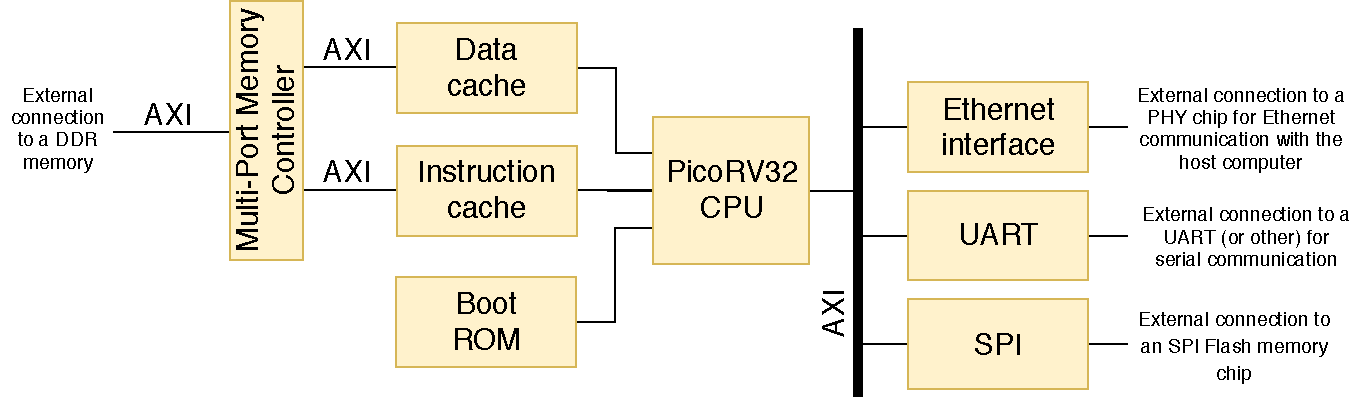
\includegraphics[width=1\linewidth]{Figures/soc2}
\caption{Top level block diagram of the \socname System on Chip.}
\label{fig:soc}
\end{figure}

The top-level topology of the \socname System on Chip is shown in
Figure~\ref{fig:soc}. \socname is intended to be build as a base SoC for future
development of IoT hardware and software systems, which means that the key
attributes of \socname must be small area, low power consumption and high
performance. Another very important feature for the \socname System on Chip and
for the development environment to be built during this project is
configurability, so to allow developers to choose which of the specifications
mentioned earlier are the most important to optimize, according to the
application intended for the SoC being developed.

As such, several RISC-V CPU alternatives were taken into account when choosing
which one of them was going to be used to build the \socname System on
Chip. Those were Rocket Chip \cite{bib:rocketchip}, Taiga \cite{bib:taiga},
PULPino \cite{bib:pulpino}, and PicoV32 \cite{bib:picorv32}. Brief descriptions
of each architecture are given next, as well as the identified reasons to
discard the ones that were not sufficiently fitting for the \socname System on
Chip.

\begin{itemize}
	
	\item \textbf{Rocket Chip} \cite{bib:rocketchip} is the de facto
          standard for SoC development using RISC-V processor cores, as it was
          made by the same team that introduced the RISC-V ISA. Rocket Chip is a
          synthesizable RTL generator that allows customization and
          parameterization of two RISC-V processor cores architectures (one
          being in-order and the other out-of-order). However, due to the fact
          that Rocket Chip has a great amount of features, it has proved to be
          too hard to manipulate in the past, so this option is put aside.
	
	\item \textbf{Taiga} \cite{bib:taiga} is a high-performance RISC-V
          softcore written in SystemVerilog, developed mainly for use in FPGAs
          and for supporting multicore configurations using an OS. However,
          given the fact that the focus of this architecture is to solely
          optimize performance and resource allocation in FPGAs, it not suited
          for the applications envisioned for this project, as the \socname
          System on Chip is meant to reach ASIC implementation.
	
	\item \textbf{PULPino} \cite{bib:pulpino} is an open source single core
          microcontroller system that can be configured to use either one of two
          different in-order and single-issue CPU architectures: RI5CY
          \cite{bib:riscy} or zero-riscy \cite{bib:zeroriscy}. Both are designed
          to be used in ultra low power \footnote{Ultra low power in eletronic
            circuits means that the transistors are operated with the minimal
            power supply possible. As such, the transistors are operated at
            sub-threshold regions, with ultra low threshold voltages.} designs
          \cite{bib:ultralowpower}.
	
	In particular, RI5CY has 4 pipeline stages, an IPC (Instructions Per
        Cycle) approximately equal to 1 \cite{bib:riscvmanual} and full support
        of the RV32I base instruction set. It supports some of the RISC-V ISA
        extensions, such as the RV32C, RV32M and RV32F and it also supports
        other ISA extensions such as fixed-point operations, dot product and
        others. RI5CY implements a subset of the privileged specification of the
        1.9 version of the RISC-V ISA~\cite{bib:riscvprivileged19}. As of the
        date of writing of this document, the latest version of the privileged
        architecture of the RISC-V instruction set is v1.10
        \cite{bib:riscvprivileged110}.
	
	The zero-riscy architecture is derived from RI5CY CPU core. It features
        2 pipeline stages and, like the RI5CY core, supports the RV32I base
        instruction set and the RV32C and RV32M extensions. It is also possible
        to reduce the number of registers to 16, configuring the zero-riscy core
        to adopt the RV32E RISC-V instruction set, which is useful for embedded
        systems. This architecture also implements a subset of the privileged
        specification of the 1.9 version of the RISC-V ISA, just like RI5CY.
	
	PULPino provides a set of peripherals such as I2S, I2C, SPI and UART for
        communication with external systems. PULPino, RI5CY and zero-riscy are
        were all written with the SystemVerilog HDL\footnote{SystemVerilog is
          also a Hardware Verification Language (HVL).} (Hardware Description
        Language).
	
	\item \textbf{PicoRV32} \cite{bib:picorv32} is a size-optimized RISC-V
          processor core that implements the RV32IMC instruction set. Although
          being small, it features a high maximum clock frequency (250-450 MHz
          on 7-Series Xilinx FPGAs, according to the README file in
          \cite{bib:picorv32}). The RV32C and RV32M extensions are supported, so
          it is possible to configure this PicoRV32 as an RV32IM, RV32IC or
          RV32IMC core. It is also possible to configure it as a RV32E core. It
          also supports other optional useful features for SoCs and embedded
          systems, such as a built-in interruption controller and a co-processor
          interface.
		
\end{itemize}

So, the two contenders for being the CPU architecture in the \socname System on
Chip are PULPino and PicoRV32. In the end, it was decided to use the PicoRV32
CPU architecture to build the \socname System on Chip. The reasons for choosing
this processor core over PULPino are the following:

\begin{enumerate}
	
\item PULPino's features, although interesting for SoC design and embedded
  systems, go beyond the scope of the project. Namely, it implements a subset of
  the RISC-V privileged ISA, which is a feature purposely left out of the
  project at hand because, for the time being, there is no interest in running
  an OS in the \socname System on Chip. Instead, a smaller set of simple custom
  instructions can be used for Interruption Request (IRQ) handling, which
  PicoRV32 already implements.

\item PicoRV32's GitHub repository is the most complete of the two, where there
  are made available some application examples of the PicoRV32 CPU, namely the
  PicoSoC example SoC and a simple system with just a CPU core and a memory unit
  connected by PicoRV32's native interface.

\item On the one hand, PicoRV32's provided testbenches in the respective GitHub
  repository delivered positive results. The simple CPU + memory system
  mentioned in the previous item was also synthesized in FPGA (details are in
  Chapter~\ref{chapter:results}). On the other hand, there were efforts in the
  past to integrate PULPino in a system being developed at IObundle, but the
  team was incapable of detaching the PULPino core from the environment where it
  was demonstrated because there was not enough information available to do so.

\end{enumerate}


%%%%%%%%%%%%%%%%%%%%%%%%%%%%%%%%%%%%%%%%%%%%%%%%%%%%%%%%%%%%%%%%%%%%%%%%
\subsection{CPU}
\label{subsection:cpu}

The CPU is the most important component of the system. It runs programs stored
in an external DRAM memory and connects to all other components\footnote{The CPU
  does not connect directly to the memory controller, but instead is connected
  through a cache interface.}.

The CPU architecture used in the \socname System of Chip is PicoRV32. It
supports the RVC standard RISC-V ISA extension and the base ISA RV32E, which are
important features for SoC development, as explained in
Subsection~\ref{subsection:userlevelisa}.

Other key features of PicoRV32 are:

\begin{itemize}
	\item Small size. When deployed on a 7-Series Xilinx FPGA, it uses
          between 750 and 2000 LookUp Tables (LUTs);
	\item Maximum frequency between 250 MHz and 450 MHz on 7-Series Xilinx
          FPGAs;
	\item CPI approximately equal to 4, but depends on the mix of
          instructions in the code. For more details, the README file
          in~\cite{bib:picorv32} should be consulted;
	\item Selectable native memory interface or AXI4-Lite master and Verilog
          description of an interface to use between two cores with different
          memory interfaces (AXI4-Lite or native);
	\item Optional IRQ support using a simple custom ISA;
	\item Optional Co-Processor Interface, which can be used to implement
          non-branching instructions in external co-processors, such as the M
          standard RISC-V ISA extension;
	\item Option to choose single-port or dual-port register file
          implementation, which can be useful to configure reduce the core's
          size or to increase it is performance;
\end{itemize}


%%%%%%%%%%%%%%%%%%%%%%%%%%%%%%%%%%%%%%%%%%%%%%%%%%%%%%%%%%%%%%%%%%%%%%%%
\subsection{Ethernet interface}
\label{subsection:ethernet}

Ethernet is a widely used communication protocol that was first commercially
introduced in 1980. Since then, it has evolved to a point where it is possible
to transfer data through Ethernet cables with bandwidths from 10 Mbit/s to 100
Gbit/s\footnote{Ethernet using more than 100 Gbit/s of bandwidth is called
  Terabit Ethernet (TbE). TbE standards for 200 Gbit/s and 400 Gbit/s Ethernet
  were developed by the IEEE P802.3bs Task Force and were approved on December
  6, 2017. However, the term Ethernet usually refers to the 10 Mbit/s to 100
  Gbit/s range, while the above ranges are referred as TbE.}. An Ethernet
interface is currently in development for a separate Versat~\cite{bib:versat}
project at IObundle, which is intended to be used in the \socname System on Chip
as well.

The Ethernet interface will be used instead of a JTAG tap for communication of
the \socname System on Chip with the host computer, with the objective of
reducing drastically the time needed to load programs into the SoC and to send
bitstreams from the host computers to FPGA where \socname is being emulated.

In the \socname System on Chip, the Ethernet interface will be connected to the
CPU via an AXI interface.


%%%%%%%%%%%%%%%%%%%%%%%%%%%%%%%%%%%%%%%%%%%%%%%%%%%%%%%%%%%%%%%%%%%%%%%%
\subsection{UART}
\label{subsection:uart}

An Universal Asynchronous Receiver-Transmitter (UART) is needed for debug and
printing purposes. A UART is a hardware device that implements the RS232 serial
protocol for data communication through two serial ports: one for transmitting
(often labeled as TX) and another for receiving (often labeled as RX). When data
transfer is taking place, the UART outputs a start byte in the TX port, followed
by the 8 bits that compose the byte that needs to be transmitted and finally a
stop bit. When receiving data, it checks if a start bit in the RX port in
received and, when detected, it receives the 8 bits and the stop bit and
converts the received serial data into a byte. So, the UART is usually used to
send char strings from the SoC to a terminal on the host computer. The UART also
has a clock divider scheme to adjust its BAUD rate.

The PicoRV32 GitHub repository already has an example SoC where a UART open
source Verilog description is included and connected to the CPU via the
PicoRV32's native memory interface. In the \socname System on Chip, the UART
will be connected to the CPU via an AXI interface.


%%%%%%%%%%%%%%%%%%%%%%%%%%%%%%%%%%%%%%%%%%%%%%%%%%%%%%%%%%%%%%%%%%%%%%%%
\subsection{SPI}
\label{subsection:spi}

A Serial Peripheral Interface (SPI) is also included to allow communication with
an SPI Flash memory unit, which can store program data destined to be transfered
to the CPU. However, the SPI can also be used to communicate with other low
speed peripherals. Similarly to the UART, the SPI is also a serial interface,
but while the UART transfers data asynchronously, the SPI offers synchronous
communication. The SPI is also much faster transferring data than the UART,
because the first can usually send data through 2, 3 or 4 wires, while the
second has only one wire available for this task.

An alternative to the SPI would be an I2C, which is also a synchronous serial
interface. However, there are numerous reasons why the SPI is preferable. The
most obvious one is that the I2C is typically slower and is more complex than
the SPI, because its hardware is based on an addressing scheme and the SPI
simply uses a chip select line. Also, SPI flash memory is the easiest and
cheapest kind of off-chip non-volatile memory available nowadays, so it is more
pertinent to consider an SPI.

The PicoRV32 GitHub repository already has an example SoC where an SPI open
source Verilog description is included and connected to the CPU via the
PicoRV32's native memory interface. In the \socname System on Chip, the SPI will
be connected to the CPU via an AXI interface.


%%%%%%%%%%%%%%%%%%%%%%%%%%%%%%%%%%%%%%%%%%%%%%%%%%%%%%%%%%%%%%%%%%%%%%%%
\subsection{Boot ROM}
\label{subsection:bootrom}

A Read-Only Memory (ROM) is typically used in computer systems to store a boot
program that is executed after each machine reset. As such, boot ROMs are
connected to the system's CPU. When the reset signal is received, it the boot
ROM loads the program to the CPU's memory and is then executed. During the
professional internship at IObundle, the author used the picoVersat controller
(i.e. Versat's~\cite{bib:versat} controller), where the boot program stored in
the boot ROM was a simple loop to check if a non-zero value was written to
register R0 (signaling that a program was ready to be executed) and, if it did,
a branch to the program memory's base address would be made, starting the
program.

In the \socname System on Chip, the boot ROM is connected to the CPU via
PicoRV32's native memory interface.


%%%%%%%%%%%%%%%%%%%%%%%%%%%%%%%%%%%%%%%%%%%%%%%%%%%%%%%%%%%%%%%%%%%%%%%%
\subsection{Multi-Port Memory Controller}
\label{subsection:memcontroller}

A DRAM controller is used to control data transfer between the external DRAM
memory and the CPU. The DRAM controller connects to the external DRAM memory and
to the data and instruction caches mentioned below through AXI interfaces, as
depicted in Figure~\ref{fig:soc}.


%%%%%%%%%%%%%%%%%%%%%%%%%%%%%%%%%%%%%%%%%%%%%%%%%%%%%%%%%%%%%%%%%%%%%%%%
\subsection{Instruction and Data Caches}
\label{subsection:caches}

Between the DRAM controller and the CPU, a data cache and an instruction cache
are present, in order to increase memory access performance. Caches are a kind
of smaller but faster memory used to interface a CPU and a RAM memory in order
to increase memory access speed. When the CPU access new data, it first checks
if the data is in the cache. If not, then the data is loaded from the RAM memory
to the cache so that the next time the processor needs to access it, it can read
or write it faster.

The caches are connected to the CPU via PicoRV32's native memory interface and
to the DRAM controller through an AXI interface.


\cleardoublepage

%%%%%%%%%%%%%%%%%%%%%%%%%%%%%%%%%%%%%%%%%%%%%%%%%%%%%%%%%%%%%%%%%%%%%%%%
%                                                                      %
%     File: Thesis_Background.tex                                      %
%     Tex Master: Thesis.tex                                           %
%                                                                      %
%     Author: Andre C. Marta                                           %
%     Last modified :  2 Jul 2015                                      %
%                                                                      %
%%%%%%%%%%%%%%%%%%%%%%%%%%%%%%%%%%%%%%%%%%%%%%%%%%%%%%%%%%%%%%%%%%%%%%%%

\chapter{SoC development}
\label{chapter:environment}

In this chapter, the verification environment and development flow of the \socname System on Chip are presented and a description of how the first can be used in the several development stages is given.

\section{SoC verification}
\label{section:verification_env}
Most of the time that takes for an IC to be developed is spent on verification i.e. running tests to see the design was correctly built. There are no systematic/general/standard methods for validating such designs that can vary much in complexity and size. Because of this, many different verification techniques are employed to test the SoC. 

\subsection{Warpbird verification environment}
Two very similar SoC verification environments that use open source components are the ones developed in \cite{bib:blackbird,bib:warpbird}. Figure~\ref{fig:env_warpbird} illustrates the one built in the Warpbird project \cite{bib:warpbird}, as it is the most recent one.

\begin{figure}[!h]
	\centering
	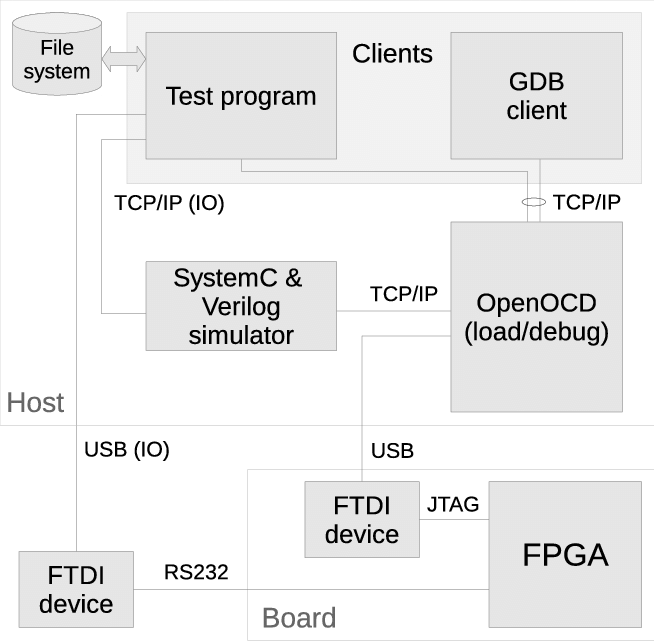
\includegraphics[width=0.5\linewidth]{Figures/env_warpbird}
	\caption{Warpbird's verification environment (figure taken from \cite{bib:warpbird}).}
	\label{fig:env_warpbird}
\end{figure}

Warpbird's verification environment is already described in \cite{bib:warpbird}, so this section will only refer and briefly detail some of its parts which contrast with the verification environment envisioned for \socname, so to emphasize the novelties introduced in respect to Warpbird.

Warpbird uses a JTAG tap which communicates with the host computer via an FTDI bridging device that translates JTAG to USB and vice-versa. The USB side of the FTDI devide then connect to OpecnOCD~\cite{bib:openocd}, an universal chip debug tool that provides a unified target access mechanism, facilitating the implementation of the communication structure between clients (such as the test program and GDB) and the FPGA.

OpenOCD allows debugging of programs running remotely on the FPGA using GDB, as if those programs were being ran locally. A test program is connected via a TCP/IP socket internal to the host machine to send OpenOCD commands such as program loading, execution halt and start, etc to the FPGA. OpenOCD is also connected via an internal TCP/IP socket to Verilator~\cite{bib:verilator} (SystemC \& Verilog simulator) to allow debugging on the RTL simulation target as well.

\subsection{\socname verification environment}
The verification environment for \socname will be based on Warpbird's. However, some adaptations must be made because the toolchains are different in the two and the two SoCs do not have the same interfaces to communicate with the outside world. For example, unlike Warpbird, \socname does not use the Rocket Chip generator and Chisel3 scala embedded language tools and has an Ethernet interface instead of a JTAG tap, which Warpbird has.

Because the JTAG tap is not used in \socname, we no longer need to use OpenOCD and the FT4232H Mini Module, which was used to bridge communications from the host machine to the JTAG pins in the FPGA board, which in turn were connected to Warpbird's JTAG tap, inside the FPGA itself. The FT2232H device\footnote{i.e. the FTDI device in the lower left corner in Figure~\ref{fig:env_warpbird}} is no longer necessary as well, because the Ethernet interface in \socname allows the clients (i.e. the test program and GDB) can communicate with the FPGA via Ethernet instead of converting USB streams from the host computer into RS232 streams to the FPGA and vice-versa.

\begin{figure}[!h]
	\centering
	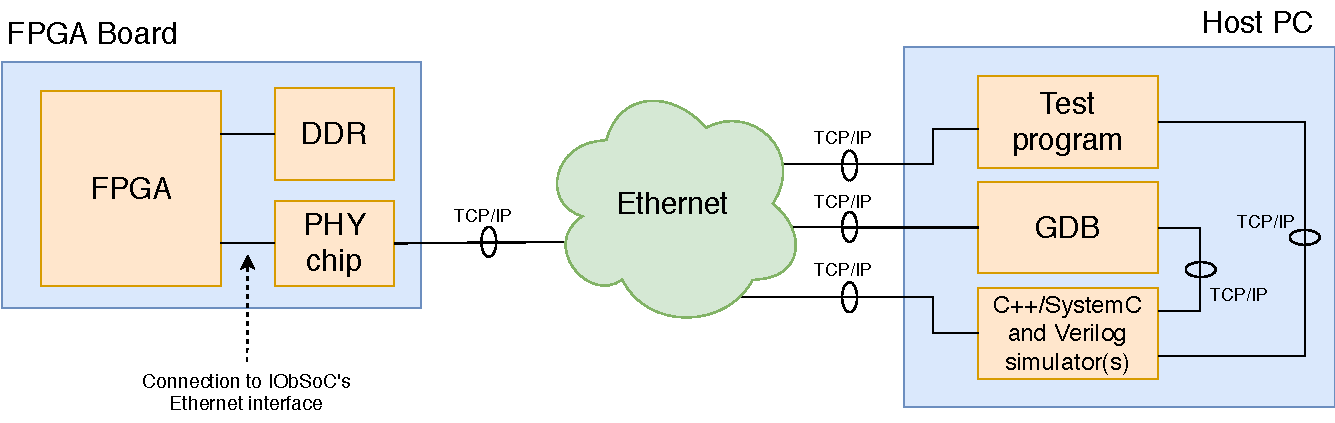
\includegraphics[width=1\linewidth]{Figures/env}
	\caption{Verification environment based on \socname.}
	\label{fig:env}
\end{figure}

Therefore, all communications between the host computer and the FPGA are now done using Ethernet, which simplifies the verification environment structure, as it can be seen in Figure~\ref{fig:env} compared to Figure~\ref{fig:env_warpbird}. On top of that, Ethernet is the most popular link-layer protocol on which TCP/IP is carried out, so this Ethernet communication infrastructure is an appealing choice. Because OpenOCD no longer exists in the verification environment, the C++/SystemC and Verilog simulator(s), the test program and the GDB client communicate directly with the FPGA via a TPC/IP socket which runs on top of an Ethernet connection. Also, GDB's communication with the simulator(s) is now done via a direct internal TCP/IP socket in the host machine, just like the one that already exists between the test program and the simulator(s).

The use of this new Ethernet infrastructure not only simplifies the verification environment but also makes communications between the host machine and the FPGA (or the SoC) much faster, because Ethernet bandwidth ranges between 10 Mbit/s and 100 Gbit/s, when JTAG's typical maximum bandwidth is several tens of Mhz. Besides this new way of communication between the host PC and the FPGA, most of the remaining structure of the verification environment will be similar to Warpbird's. 

After peripherals are added to \socname, SoC verification begins with RTL simulation, where dedicated testbenches and test programs are produced to test and evaluate it (these topics are better described in Section~\ref{section:devel_flow}). The simulators considered to integrate this environment are:

\begin{itemize}
	\item \textbf{Verilator}~\cite{bib:verilator}, which converts the Verilog description the SoC design to a C++/SystemC equivalent cycle-accurate behavioral model. This allows fast simulation of complex and large systems, but limits the truth values to 0 and 1, whereas other simulators use Z (high impedance), U (undefined) and others. Verilator is free and open source;
	
	\item \textbf{Icarus Verilog}, which is an open source simulation and synthesis tool more suited for small or medium-small sized projects. For medium to large-sized projects, a proprietary simulator or Verilator are better options, as Icarus becomes too slow, which may lead to project delays;
	
	% UM DOS OBJETIVOS É QUE O AMBIENTE DE DESENVOLVIMENTO SEJA OPEN SOURCE, POR ISSO NÃO SEI SE O NCSIM DEVE SER REFERIDO OU NÃO.
	\item \textbf{NCsim}, a commercial proprietary simulation engine contained in Cadence's design and verification tools suite. Although proprietary and very expensive, such a simulation tool may sometimes be necessary for large projects to be completed in a reasonable time window. Instituto Superior T\'{e}cnico makes NCSim available in machines that can be remotely accessed by students, professors and researchers at the university. The licenses for NCSim are payed with the help on European Union (EU) funds.
\end{itemize}

The waveforms generated by the simulations are then viewed in a waveform viewer such as GTKWave (a free waveform viewer). If errors are encountered, the SoC design must be rectified and new RTL simulations need to be made. After obtaining the expected results, the second step of the verification process is to target an FPGA and implement the SoC. When a bitstream is successfully generated, deployment of the SoC in the FPGA is made and tests are made in the FPGA emulated SoC. Every time unexpected problems occur, the verification needs to take a step back to the previous phases until all problems are solved. In each development stage that uses the verification environment\footnote{As it will be described in Section~\ref{section:devel_flow}, all development stages except in the first one, which is the toolchain installation.}, after successfully deploying the SoC in the FPGA, development advances to the next stage.

Another detail to account for is that because \socname does not have a debug module (unlike Warpbird), it is necessary to develop software to implement useful (and some indispensable) debug commands such as break, run, halt, continue, peek and poke. This debug program will be stored in the external DDR memory.


%%%%%%%%%%%%%%%%%%%%%%%%%%%%%%%%%%%%%%%%%%%%%%%%%%%%%%%%%%%%%%%%%%%%%%%%

\section{Development flow}
\label{section:devel_flow}
The development flow in which the SoC development environment will be based is the same as the one used in \cite{bib:blackbird,bib:warpbird}, which is illustrated in Figure~\ref{fig:devflow}.

\begin{figure}[!h]
	\centering
	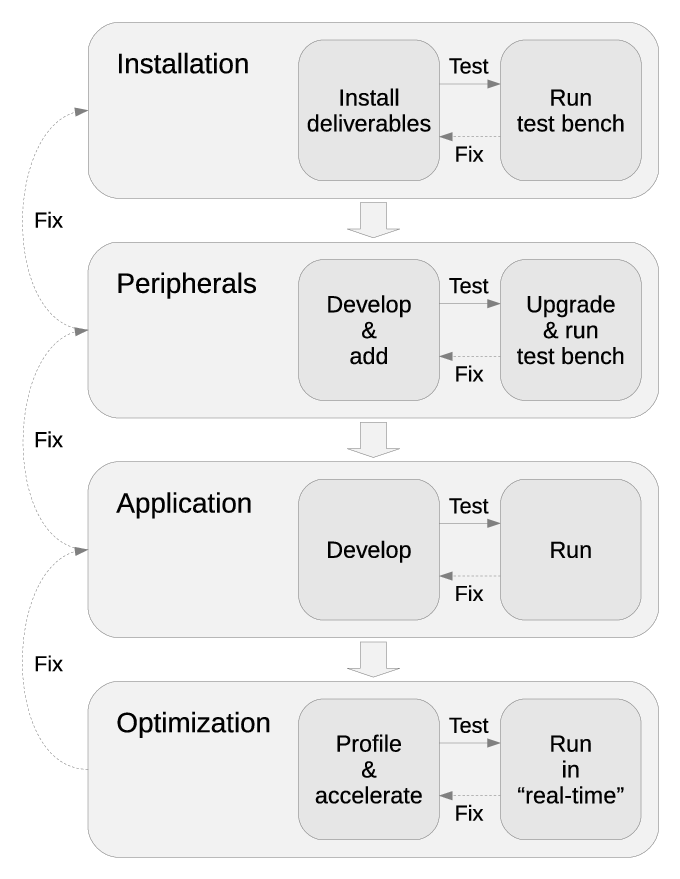
\includegraphics[width=0.5\linewidth]{Figures/devflow}
	\caption{Development flow (figure taken from \cite{bib:blackbird}).}
	\label{fig:devflow}
\end{figure}

\subsection{Toolchain installation}

%referir que as makefiles do picorv32 permitem instalar rapidamente o subconjunto necessario da toolchain do risc-v para que os testbenches básicos %corram sem problemas. Instala outras coisas, ver melhor o que (talvez o verilator?)
%listar algumas coisas to toolchain do risc-v que são instaladas para o picorv
%fazer uma lista de todas as ferramentas instaladas

The first stage of the development flow is the installation of the tools necessary to develop the SoC, such as compiler, assemblers, linkers, simulators and others. The PicoRV32's GitHub repository~\cite{bib:picorv32} provides a Makefile script to install the complete RISC-V toolchain. However, it is not necessary to install all of its tools, as some are not used by PicoRV32. 

The default settings of the build scripts available in the riscv-tools repository~\cite{bib:riscvtools} build a compiler, assembler and linker that can target any RISC-V ISA. However, the libraries are built for RV32G and RV64G targets. For this reason, the README file in PicoRV32's GitHub repository~\cite{bib:picorv32} also provides instructions with Linux shell and make commands to install a pure RV32I, RV32IC, RV32IM or RV32IMC CPU (including libraries). These commands include:

\begin{enumerate}
	\item the installation of various software packages\footnote{The list of packages installed can be seen in the shell commands provided in \cite{bib:picorv32}, in the \textit{Building a pure RV32I Toolchain} topic.};
	\item the creation of the installation directory inside the /opt folder;
	\item the download of the RISC-V GNU toolchain from \cite{bib:riscvgnutools} using git commands;
	\item building the toolchain in the host machine with a configure script.
\end{enumerate}

After installing the toolchain, a testbench is ran with standard configurations to check if the former was correctly installed. The testbench uses the Icarus Verilog simulation and synthesis tool ~\cite{bib:icarus}. There is also a simpler testbench that does not require an external firmware .hex file, which can be useful in systems that do not have the RISC-V compiler toolchain installed.

\subsection{Adding peripherals to \socname}
In the second stage of development, SoC components are added to \socname by describing them with the Verilog HDL. The example projects' files provided in PicoRV32's GitHub repository \cite{bib:picorv32} can provide helpful guidelines for this task. The peripherals to be added can be used as co-processors using PicoRV32's Pico Co-Processor Interface (PCPI) or can simply be connected to a PicoRV32 core through the AXI4-Lite memory interface provided. More PicoRV32 cores can be instantiated and interconnected using its native memory interface.

The standard RISC-V ISA extensions supported by PicoV32 can be added by turning on Verilog \textit{`define} flags in PicoRV32's Verilog description file (picorv32.v). When used, the multiply core provided in the repository in connected to PicoRV32 through the PCPI interface. One must remember to active the PCPI interface enable flag for the multiply core to work.

% ACHO QUE NÃO DOMINO SUFICIENTEMENTE BEM ESTES PORMENORES PARA FALAR BEM DELES...
% When new hardware or software components are added, the cross-compiler needs to become aware of the new hardware. There are options to make the compilation aware of new hardware units.

The verification environment described in Section~\ref{section:verification_env} is used to test the new SoC components. After being sure the peripherals are correctly connected and working, the SoC development may advance to the next stage.

\subsection{Application development}
Next, the software application to be ran in the SoC's CPU is developed using an IDE. Since no IDE integration is provided, the IDE can be chosen by the company or developer. The application can be ran in the verilated model of the SoC (i.e., the equivalent C++/SystemC model obtained with Verilator), generating cycle-accurate results, and in the FPGA emulated SoC, which is faster and more accurate. Debugging the application in both targets using GDB is also possible. These features are already detailed in Section~\ref{section:verification_env}.

The verification environment is once again used in this development stage in order to test the software application. After assuring the software implements the desired functionality, development advances to the final stage.

\subsection{Optimization}
The final development stage consists on optimizing the application developed in the previous stage. In order optimize software applications, profilers are used. A profiler is a dynamic program analysis tool that measures, for example, the frequency and duration of each function call in a program, the usage of instructions (i.e., the total number of times an instruction is used) and the memory space and time complexities of a program. This allow the software developer to understand which aspects or code blocks are affecting performance the most, identifying more easily the software components that should be priorly optimized.

The RISC-V toolchain does not have a profiler available. A way to work around this issue in software development using C or C++ is to use timing libraries such as time.h or other more appropriate ones to a targeted FPGA board to measure the time duration of each function call. Furthermore, for easing the use of this feature, one can use the pre-build compiler directives to turn the time measure feature on and off by simply uncommenting or commenting a compiler flag definition. An example is provided in the following piece of C code:
\begin{lstlisting}[frame=single,basicstyle=\footnotesize\ttfamily,linewidth=\columnwidth,breaklines=true,language=C]
#define COUNT_TIME // comment/uncomment this line to shut off/on time measure feature

// more code

#ifdef COUNT_TIME
start_time_count_routine();  // assume time duration value's mem. space is selected here
#endif
some_function_call();
#ifdef COUNT_TIME
finish_time_count_routine(); // assume time duration value is stored here 
#endif

// more code
\end{lstlisting}
\cleardoublepage

%%%%%%%%%%%%%%%%%%%%%%%%%%%%%%%%%%%%%%%%%%%%%%%%%%%%%%%%%%%%%%%%%%%%%%%%
%                                                                      %
%     File: Thesis_Results.tex                                         %
%     Tex Master: Thesis.tex                                           %
%                                                                      %
%     Author: Gonçalo Santos                                           %
%     Last modified : 20 Oct 2018                                      %
%                                                                      %
%%%%%%%%%%%%%%%%%%%%%%%%%%%%%%%%%%%%%%%%%%%%%%%%%%%%%%%%%%%%%%%%%%%%%%%%

\chapter{Results}
\label{chapter:results}

The aim of this work is to produce a workable {\bf C} language
compiler for the {\it Versat} architecture using the {\it picoVersat}
instruction set.
The success can be measured by the number of {\bf C} language
constructs that are working properly.
Consequently, testing is of primordial importance, as are the range
of tests used to exercise the compiler.

\section{Functionality}

The compiler, as far the tests were comprehensive,
supports all {\bf C} language integer constructs.
Limitations are listed below.

Since the processor instruction set is reduced, as are the
number of {\bf lcc} terminals to be implemented by the compiler,
the testing of each operation, on its own, is strait
forward.
Testing sequences of such operations may prove more
difficult to test, since different {\bf C} programs
can produce different selection matches.

\section{Testing}

In the test of a compiler, where a small change can affect the
generation of multiple instructions, a good set of
regressive tests is very important.
In order to automate the process, a {\tt test/} directory
was setup.
This directory includes a set of {\bf .c} test files and
the expected output {\bf .out}.

The {\tt Makefile} compiles, executes and compares the new
result with the previously stored result.
All differences in output are printed and can then be analyzed.

Since the output from {\bf iverilog} includes the number
of clocks spent, it is easy to compare whether the changes in the
compiler result in improvements, or in performance degradation.

Some tests are very simple and its output can be easily predicted.
To make testing even simpler, the return value of the {\tt main}
routine is printed, unless the {\sc NORET} environment variables
is defined. Upon return from the {\tt main} routine, the lowest
nibble is printed as an {\sc ASCII} starting at $0$.
This means that values between $10$ and $15$ are printed as
the {\sc ASCII} character at the respective offset, namely the
sequence: \verb|:|, \verb|;|, \verb|<|, \verb|=|, \verb|>|, \verb|?|.

More complex tests can be compiled with {\bf gcc} and executed
to access the expected output.
This, however, can not be performed if the examples include
{\tt asm} calls, since the code can only be executed by the
{\it Versat}, or by the {\bf iverilog} simulator, and not by the
native testbench processor.
%vdb.c

A set of $86$ regression tests is currently being used, ranging
from specific operator testing to complex recursive and iterative
examples. % And the number of tests keeps growing ...

\section{Limitations}\label{limitations}

The {\bf C} language imposes that {\tt sizeof(char)==1}
as does the {\bf lcc} compiler (see~\cite[p.79]{hanson95}).
This works fine as far as {\tt sizeof(char)} can be 32-bits.
However, additionally, the {\bf lcc} assumes through out
the code that $8$ is the number of {\em bit-per-byte}.
If it was a variable, one could set it to $32$.
As it is hardcoded, all address literals
will be truncated to 8-bits ({\tt 8}${}^{\wedge}${\tt ty->size}).
\begin{verbatim}
int *addr = (int*)0x123456;
\end{verbatim}
This can be avoided by setting an integer to the
required value and then assigning it to a pointer.
This works since integer literals are 32-bit wide
and the conversion to pointer, controlled by the
{\it back-end}, does not truncate the value.
\begin{verbatim}
int *addr, value = 0x123456;
addr = (int*)value;
\end{verbatim}
Nevertheless, defining literal pointer is never
a good predictive in virtual memory machines.
In {\it Versat} it is useful to map variables
to specific addresses.

Due to the same reason, a warning message is issued
({\tt shifting an `int' by 12 bits is undefined})
but the code is correctly generated.

% #define LONG_MIN -2147483648
% warning: unsigned operand of unary -
% but 0x80000000 or bellow is OK!
% #  define LONG_MAX	2147483647
% #  define LONG_MIN	(-LONG_MAX - 1L)

In the initial version of {\it picoVersat}, all global
data must be added by {\tt MEM\_BASE=512}.
Since this is performed when addresses are fetched,
static assignments store the unadded value.
Therefore, all accesses must be added by $512$.
Must add {\tt 512} to global pointers in {\tt picoversat-0.0}
\begin{verbatim}
int mem[10], *base = mem;
int main() { base[6+512] = 9; return return mem[6]; }
\end{verbatim}
This can be avoided if assignment is performed during
execution (not at compile time), even if the variable
is global.
\begin{verbatim}
int mem[10];
int main() { int *base = mem; base[6] = 9; return return mem[6]; }
\end{verbatim}

Signed multiplication, division and modulus ({\tt \_mul},
{\tt \_div} and {\tt \_mod}) do not generate carry since
the flags register of {\it picoVersat} is read-only.

The {\bf C} programming languages relies on separate
compilation, where several files are independently
compiled and then linked together.
However, there is no linker in the {\it Versat} system
and the assembler {\bf va} does not support multiple
files.
The solution is to perform linking with {\bf cpp} %%%
include directives.
While in normal {\bf C} the {\tt .c} should be
included, rather compiled, the inclusion of {\bf .h}
as well as {\bf .c} accomplishes the desired result.
Since there is no linking, only multiple inclusion
of files must be avoided.

The {\it Versat} architecture is meant to be used offline
and no form of argument passing to the {\tt main} routine
is available.
Consequently, the stack is initialized at the top.
Therefor, even if the program declares arguments to
the {\tt main} routine ({\tt argc, argv, envp}) they should
never be accessed.
Also, since the system has no memory management unit,
all illegal accesses are silently ignored by the system.
Highly recursive routines that exhaust the stack will have
unpredictable behaviors, since they will begin to overwrite
the top of the code.
Even if it is not the compilers responsibility, it something
that the programmer should be aware, especially when
transitioning from a virtual managed memory system.

Finally, the compiler does not support floating point
data types, since every operation must be supported
by library routines.
This is the case for many android devices, namely
smartphones.
However, the {\it Versat} purpose is to perform
integer arithmetic operations fast and is not aimed at
scientific programming.
The error message {\tt compiler error in \_label--Bad terminal}
is issued by the compiler when it cannot handle a given operation,
namely floating point operations.

\section{Register assignment}

Register assignment in compiler design considers two types of registers:
global registers that hold variable values and scratch registers that hold
temporary values.
The {\bf lcc} compiler defines these registers by setting a mask for each
type of register.
It is up to each {\it back-end} to define the mask values according to processor
capabilities.
For instance, the {\bf sparc} processor defines $4$ sets of $8$ registers:
global, temporary, input and output; where the later two sets replace
the stack for argument passing.
In {\bf i386} all $7$ registers are temporary, while {\bf mips} uses half
for each purpose ($16+16$).

Since the {\it picoVersat} has no specific register assignment, a study
was carried out in order to assess the best balance between global and
scratch registers.
Registers {\tt R0} and {\tt R13} to {\tt R15} are used to communicate with {\it Versat}
and are invisible to the compiler.
The stack is controlled by a {\it stack pointer} ({\tt R12}) and a {\it frame pointer}
({\tt R11}).
The remaining registers ({\tt R1} to {\tt R10}) compose a mask {\tt 7FE}, where
the lowest bit ({\tt R0}) is omitted for register assignment, and the highest
used bit {\tt 400} is {\tt R10}.
The register {\tt R1} is used to return function values and all arguments are
passed on the stack.
At least two registers must be used as scratch for binary operations
temporaries.
The compiler allows the definition of a {\tt tmask} for temporaries and a
{\tt vmask} for variables.

Initially, in run $1$, the experiment uses all registers for temporaries.
Each run adds a variable register at the expense of a temporary, until only
two temporaries remain (run $9$).
Three examples where used: {\tt assign}, {\tt repeating locals} and
{\tt bubble sort}.
The first two represent opposite extremes of register usage, while the last is
a more balanced and realistic example.

The first example uses the {\bf C} language right associative {\it assign} operator
where each new assignment to the variable {\tt a} requires a new temporary register.
%(see Figure~\ref{fig:assign}).

%\begin{figure}
\begin{verbatim}
int f() { return 1; }
int main()
{
  int a;

  a = f() + (a =
      f() + (a =
      f() + (a =
      f() + (a =
      f() + (a =
      f() + (a =
      f() + (a =
      f() + (a =
      f() + (a =
      f() + (a =
      f() + (a =
      f() + (a =
      f() + (a = 1
                  )))))))))))));
  return a;
}
\end{verbatim}
%\caption{}
%\end{figure}

The register usage shows that each assign uses a register $4$ times at
the expense of the return register {\tt R1}.
The best solution, represented by the lowest clock count,
is to use only two temporaries, since more variables imply more stack ({\tt R12}),
saves and restores between each call to the function {\bf f}.

%\begin{table}
\begin{center}
{\small
\begin{tabular}{r|r|r|r|r|r|r|r|r|r|r|r|r|r|r|r|r}
run&vars&vmask&tmask&R1&R2&R3&R4&R5&R6&R7&R8&R9&R10&R11&R12&clks\\\hline
1&0&000&7FE&21&4&4&4&4&4&4&4&6&44&27&82&677\\
2&1&400&3FE&23&4&4&4&4&4&4&6&42&17&14&82&638\\
3&2&600&1FE&25&4&4&4&4&4&6&42&0&17&16&77&633\\
4&3&700&0FE&27&4&4&4&4&6&42&0&0&17&18&72&628\\
5&4&780&07E&29&4&4&4&6&42&0&0&0&17&20&67&623\\
6&5&7C0&03E&31&4&4&6&42&0&0&0&0&17&22&62&618\\
7&6&7E0&01E&33&4&6&42&0&0&0&0&0&17&24&57&613\\
8&7&7F0&00E&35&6&42&0&0&0&0&0&0&17&26&52&608\\
9&8&7F8&006&39&42&0&0&0&0&0&0&0&17&28&47&603\\
\end{tabular}
}
\end{center}
%\caption{}
%\end{table}
\vspace*{5mm}

The second example uses lots of repeating local variables so that each one is assigned
a register, for its uses from the first to last line, if one is available.
%(see Figure~\ref{fig:locals}).

%\begin{figure}
\begin{verbatim}
int func(int a, int b, int c, int d, int e, int f, int g, int h, int i, int j, int k) {
    a = a + b - c - d - e + f - g + h + i + j + k;
    b = a - b + c + d - e - f + g - h + i - j - k;
    c = a + b - c - d + e + f + g - h + i + j - k;
    d = a - b - c + d - e + f - g + h - i - j - k;
    e = a + b + c - d - e - f - g + h - i + j - k;
    f = a - b - c + d - e + f + g - h - i - j + k;
    g = a + b - c - d + e + f + g - h + i + j - k;
    h = a - b + c + d - e - f - g + h + i - j - k;
    i = a + b - c - d - e + f + g + h + i + j - k;
    j = a - b - c + d - e + f + g - h - i - j - k;
    k = a + b + c - d + e - f - g - h - i + j + k;
    return a + b + c + d + e + f - g + h - i + j - k;
}

int main() {
    return func(10, 9, 8, 7, 6, 5, 4, 3, 2, 1, 0);
}
\end{verbatim}
%\caption{}
%\end{figure}

As expected, the best solution is to use highest of temporaries in order
to reduce frame pointer ({\tt R11}) accesses to stack saved values.

%\begin{table}
\begin{center}
{\small
\begin{tabular}{r|r|r|r|r|r|r|r|r|r|r|r|r|r|r|r|r}
run&vars&vmask&tmask&R1&R2&R3&R4&R5&R6&R7&R8&R9&R10&R11&R12&clks\\\hline
1&0&000&7FE&45&27&12&13&48&46&40&45&54&62&68&56&956\\
2&1&400&3FE&53&31&13&54&46&40&47&54&62&0&78&51&1001\\
3&2&600&1FE&61&35&52&46&48&49&56&62&0&0&89&46&1051\\
4&3&700&0FE&89&39&59&63&51&56&62&0&0&0&101&41&1106\\
5&4&780&07E&109&43&75&49&74&79&0&0&0&0&113&36&1161\\
6&5&7C0&03E&146&45&84&58&105&0&0&0&0&0&124&31&1211\\
7&6&7E0&01E&156&88&112&94&0&0&0&0&0&0&138&26&1278\\
8&7&7F0&00E&171&117&176&0&0&0&0&0&0&0&154&21&1356\\
9&8&7F8&006&231&249&0&0&0&0&0&0&0&0&172&16&1447\\
\end{tabular}
}
\end{center}
%\caption{}
%\end{table}
\vspace*{5mm}

The last example, the {\it bubble sort}, uses a mixture temporaries and variable
reuses. %(see Figure~\ref{fig:bubble}).

%\begin{figure}
\begin{verbatim}
#include "printi.h"

int bubble(int list[], int n) {
    int c, d, t, swap, cnt = 0;

    for (c = 0; c < n - 1; c++) {
        for (swap = 0, d = n - 1; d > c; d--)
            if (list[d - 1] > list[d]) {    /* Swapping */
                swap++;
                t = list[d];
                list[d] = list[d - 1];
                list[d - 1] = t;
            }
        if (!swap)
            break;
        cnt++;
    }
    return cnt;
}

int v[] = { 7, 4, 9, 6, 2, 1, 3, 5, 8, 0 };

int main() {
    int i, size = sizeof(v) / sizeof(v[0]), cnt = bubble(v, size);
    for (i = 0; i < size; i++) {
        putchar(v[i] + '0');
        putchar(' ');
    }
    printi(cnt, 10);
    putchar('\n');
    return 0;
}
\end{verbatim}
%\caption{}
%\end{figure}

This example exploits the tradeoff between global and temporary register
usage.
In the first runs the compiler is unable to use all temporaries.
In the last runs some variable registers are left unassigned and the number
of required execution clocks rises again.

%\begin{table}
\begin{center}
{\small
\begin{tabular}{r|r|r|r|r|r|r|r|r|r|r|r|r|r|r|r|r}
run&vars&vmask&tmask&R1&R2&R3&R4&R5&R6&R7&R8&R9&R10&R11&R12&clks\\\hline
1&0&000&7FE&2&0&0&0&0&4&5&15&30&45&31&36&9855\\
2&1&400&3FE&2&0&0&0&0&4&7&29&41&11&24&36&8193\\
3&2&600&1FE&2&0&0&0&4&5&27&37&7&11&19&41&7714\\
4&3&700&0FE&2&0&0&0&5&25&37&4&7&11&17&41&7399\\
5&4&780&07E&2&0&0&5&19&37&6&4&7&11&13&46&7022\\
6&5&7C0&03E&2&0&5&19&33&6&6&4&7&11&9&49&6949\\
7&6&7E0&01E&2&5&19&33&0&6&6&4&7&11&9&49&6949\\
8&7&7F0&00E&5&19&33&0&0&6&6&4&7&11&9&44&6921\\
9&8&7F8&006&21&28&0&0&0&6&6&4&7&11&13&41&7492\\
\end{tabular}
}
\end{center}
%\caption{}
%\end{table}
\vspace*{5mm}

Based on experience with the examples above, a balanced approach should work best
in most cases.
Therefor, the first five registers, {\tt R1} to {\tt R5}, are used as temporaries
({\tt tmask=0x003E}) and the remaining five, {\tt R6} to {\tt R10}, are used as
variables ({\tt vmask=0x07C0}).

\section{Efficiency considerations}

Calls are very expensive operations for any processor.
{\it Intel Inc.} has made a significant effort over the year to address this
problem.
In the last years, its high end processors provide faster {\it calls} than
{\it jumps} at the expense of higher transistor count. %ref!
In a processor like {\it picoVersat}, the problem is magnified since
no stack specific registers or opcodes are available.

A function call in the {\bf C} programming language requires:
\begin{enumerate} \itemsep0em 
\item {\bf argument passing} by pushing values to the stack;
\item {\bf calling} the desired routine;
\item {\bf saving used registers} before the routine destroys its values;
\item {\bf frame pointer} saving to access arguments and locals;
\item {\bf allocate space} for local variables;
\item actually performing the routine operations;
\item {\bf restoring frame pointer} of the previous routine;
\item {\bf restoring used registers} previous values;
\item {\bf returning} to the calling routine;
\item {\bf removing arguments} from stack.
\end{enumerate}
The present compiler detects when a routine accesses no arguments or locals
and does not emit frame pointer code. So, if a routine only uses global
variables, the call becomes a bit more efficient.
Some of the tests used become upto 5\% faster by removing the frame
pointer in routines where it not needed.

As any routine can be called many times, even recursively, the compiler
must save, at the beginning, and restore, at the end,
all the registers the routine uses.
This means that, at the start of the program, the {\tt main} routine will spill
all registers it will use, although they have no defined value.
Such procedure is required since the routine may be recursively called.
However, in most cases, the {\tt main} routine is only invoked once, at
the start of the program.
The {\sc NOSAV} environment variable can be set if the {\tt main}
routine is not used recursively and no registers will saved by the compiler.
This special hack can be dangerous to use, but it makes {\tt main} based
programs more efficient.

The {\it picoVersat} controls {\it Versat} by setting specific values to
predefined memory positions.
The use of a routine to perform such a task is a very
expensive way to change memory positions, either through {\tt asm}
directives or standard {\bf C} code, as the tests {\tt set.c} and
{\tt setvar.c} show, respectively.
Memory values can be efficiently changed by assigning to a pointer
{\tt *addr=val} (see Limitations, above).

During this work, the {\it picoVersat} evolved. The use of a single
memory, for program code and data, removed the need for a {\tt addi MEM\_BASE}
instruction for each variable load and store, resulting in a 5\% improvement
over all the regression test in use, at the time. % 17022/16213 pico-0

Finally, the compiler some times generates a register read after the
same register was written by another instruction selection.
At least, the read can be suppressed, but {\bf lcc} provides no
peephole optimizer for final code cleanup.

\section{Compiler instalation}

The compiler itself, {\bf lcc}, can be invoqued directly with the
{\tt -target=versat} option, as long as the input file has already
been preprocessed ({\bf cpp}).
The compiler output is a {\it picoVersat} assembly, that can then
fed to the {\it versat} assembler ({\bf va}).

However, the complete compilation process, from {\bf C} language
source file to {\bf iverilog} simulation executable, can be
integrated as in a standard high-level compiler.

Section~\ref{app:integ} describes the requirements for such an integration.
The compiler {\tt Makefile}s, in the main and {\tt versat/} directories,
can be used to provide the instalation of all required files
for a complete development environment.
By default, without any changes to the {\tt Makefile}s, the
compiler development environment is placed under the
{\tt /usr/local/versat} directory.

The default directories for the compiler installation
({\tt make install}) are predefined as
{\tt /usr/local/versat/lcc} for the compiler files
({\tt lcc}, {\tt cpp}, {\tt rcc}, {\tt va}, and
{\tt xdict.json}), and can be redefined at compile
time or using the {\sc LCCDIR} environment variable
at runtime. The {\it picoVersat} {\tt rtl/} files
({\tt include/}, {\tt src/}, and {\tt testbench/})
should be copied to {\tt /usr/local/versat/pico}
(defined at compile time).
Also the {\bf iverilog} compiler is defined at
compile time as residing in {\tt /usr/local/bin/}.

The structure of the installed files,
in the current version is:
\begin{Verbatim}[baselinestretch=1.0]
/usr/local/versat/lcc/lcc
/usr/local/versat/lcc/cpp
/usr/local/versat/lcc/rcc
/usr/local/versat/lcc/va
/usr/local/versat/lcc/xdict.json
/usr/local/versat/lcc/include/strlen.h
/usr/local/versat/lcc/include/umod.h
/usr/local/versat/lcc/include/errno.h
/usr/local/versat/lcc/include/malloc.h
/usr/local/versat/lcc/include/umul.h
/usr/local/versat/lcc/include/itoa.h
/usr/local/versat/lcc/include/Makefile
/usr/local/versat/lcc/include/stdarg.h
/usr/local/versat/lcc/include/mem_ends.h
/usr/local/versat/lcc/include/xdict.h
/usr/local/versat/lcc/include/atoi.h
/usr/local/versat/lcc/include/puts.h
/usr/local/versat/lcc/include/dma.h
/usr/local/versat/lcc/include/versat.h
/usr/local/versat/lcc/include/ends.h
/usr/local/versat/lcc/include/mul.h
/usr/local/versat/lcc/include/xdictinc
/usr/local/versat/lcc/include/div.h
/usr/local/versat/lcc/include/ends.cbc
/usr/local/versat/lcc/include/udiv.h
/usr/local/versat/lcc/include/printf.h
/usr/local/versat/lcc/include/mod.h
/usr/local/versat/lcc/include/alloca.h
/usr/local/versat/lcc/include/printi.h
/usr/local/versat/lcc/include/gnuc.h
/usr/local/versat/lcc/include/putchar.h
/usr/local/versat/lcc/include/assign.h
/usr/local/versat/pico/testbench/sim_xtop.cpp
/usr/local/versat/pico/testbench/xtop_tb.v
/usr/local/versat/pico/include/xdefs.vh
/usr/local/versat/pico/src/xaddr_decoder.v
/usr/local/versat/pico/src/xctrl.v
/usr/local/versat/pico/src/xram.v
/usr/local/versat/pico/src/xregf.v
/usr/local/versat/pico/src/xcprint.v
/usr/local/versat/pico/src/xtop.v
\end{Verbatim}

After adding the {\tt /usr/local/versat/lcc} directory to
the {\sc PATH} environment variable, an executable example
can be produced with the command:\\
{\tt lcc example.c -o example}

The example can then be run with:\\
{\tt ./example}

Please note that the {\it versat} memory dump {\tt .hex}
file is stored in the {\tt /tmp} directory.

\cleardoublepage
 % file "Thesis_Preliminary_Results.tex"
\cleardoublepage

%%%%%%%%%%%%%%%%%%%%%%%%%%%%%%%%%%%%%%%%%%%%%%%%%%%%%%%%%%%%%%%%%%%%%%%%
%                                                                      %
%     File: Thesis_Conclusions.tex                                     %
%     Tex Master: Thesis.tex                                           %
%                                                                      %
%     Author: Carlos A. Rodrigues                                      %
%     Last modified : 21 Jan 2011                                      %
%                                                                      %
%%%%%%%%%%%%%%%%%%%%%%%%%%%%%%%%%%%%%%%%%%%%%%%%%%%%%%%%%%%%%%%%%%%%%%%%

\chapter{Conclusão}
\label{chapter:conclusao}

Insert your chapter material here...


% ----------------------------------------------------------------------
\section{Achievements}
\label{section:achievements}

The major achievements of the present work...


% ----------------------------------------------------------------------
\section{Trabalho Futuro}
\label{section:futuro}

dese


\cleardoublepage

 % file "Thesis_Conclusions.tex"
\cleardoublepage

% ----------------------------------------------------------------------
%  Bibliography
% ----------------------------------------------------------------------

% Add entry in the table of contents as chapter
\phantomsection
\addcontentsline{toc}{chapter}{\bibname}

% Include all references in .bib file, even non-cited ones...
%\nocite{*} % this should be used carefully because it is not correct!

% Produces the bibliography section when processed by BibTeX
%
% Bibliography style
% > entries ordered alphabetically
%\bibliographystyle{plain}
% > unsorted with entries appearing in the order in which the citations appear.
%\bibliographystyle{unsrt}
% > entries ordered alphabetically, with first names and names of journals and months abbreviated
%\bibliographystyle{abbrv}
% > entries ordered alphabetically, with reference markers based on authors' initials and publication year
%\bibliographystyle{alpha}
%
% Replacement bibliography styles provided by 'natbib' package
% (plainnat.bst, abbrvnat.bst, unsrtnat.bst )
% > entries ordered alphabetically
%\bibliographystyle{plainnat}
% > unsorted with entries appearing in the order in which the citations appear.
%\bibliographystyle{unsrtnat}
% > entries ordered alphabetically, with first names and names of journals and months abbreviated
%\bibliographystyle{abbrvnat} % <<<<< SELECT IF USING REFERENCES BY AUTHOR/YEAR
% > entries ordered alphabetically, with reference markers based on authors' initials and publication year
%\bibliographystyle{alpha}
%
% Custom bibliography style adapted from 'natbib' package
%   (based on http://tex.stackexchange.com/questions/5053/is-it-possible-to-get-unsrt-abbrv-bibliography)
%   (unsrtnat.bst + abbrvnat.bst -> abbrvunsrtnat.bst)
%   (original files copied from:
%   http://tug.ctan.org/macros/latex/contrib/natbib/abbrvnat.bst
%   http://tug.ctan.org/macros/latex/contrib/natbib/unsrtnat.bst
% > unsorted with entries appearing in the order in which the citations appear, with first names and names of journals and months abbreviated.
\bibliographystyle{abbrvunsrtnat} % <<<<< SELECT IF USING REFERENCES BY NUMBER (CITATION ORDER)

% External bibliography database file in the BibTeX format
\bibliography{Thesis_bib_DB} % file "Thesis_bib_DB.bib"

\cleardoublepage

% ----------------------------------------------------------------------
%  Appendix (optional)
%
%  CAUTION: 1) the main document (up to the conclusions) shall not exceed 80 pages
%           2) the document shall not exceed a total of 100 pages (per IST regulations)
% ----------------------------------------------------------------------
%\appendix

% add page number prefix according to apendix chapter (optional)
%\renewcommand{\thepage}{\thechapter.\arabic{page}}

% re-set arabic numbering (A.1,A.2,...) (optional, use only if chapter prefix is added)
%\setcounter{page}{1}

%%%%%%%%%%%%%%%%%%%%%%%%%%%%%%%%%%%%%%%%%%%%%%%%%%%%%%%%%%%%%%%%%%%%%%%%%
%                                                                      %
%     File: Thesis_Appendix_A.tex                                      %
%     Tex Master: Thesis.tex                                           %
%                                                                      %
%     Author: Andre C. Marta                                           %
%     Last modified :  2 Jul 2015                                      %
%                                                                      %
%%%%%%%%%%%%%%%%%%%%%%%%%%%%%%%%%%%%%%%%%%%%%%%%%%%%%%%%%%%%%%%%%%%%%%%%

\chapter{Vector calculus}
\label{chapter:appendixVectors}

In case an appendix if deemed necessary, the document cannot exceed a total of 100 pages...

Some definitions and vector identities are listed in the section below.

% ----------------------------------------------------------------------
\section{Vector identities}
\label{section:vectorIdentities}

\begin{equation}
	\nabla \times \left( \nabla \phi \right) = 0
	\label{eq:cross_nnp}
\end{equation}

\begin{equation}
	\nabla \cdot \left( \nabla \times {\bf u} \right) = 0
	\label{eq:dotCross_nnu}
\end{equation}

 % file "Thesis_Appendix_A.tex"
%\cleardoublepage

% re-set arabic numbering (B.1,B.2,...) (optional, use only if chapter prefix is added)
%\setcounter{page}{1}

%%%%%%%%%%%%%%%%%%%%%%%%%%%%%%%%%%%%%%%%%%%%%%%%%%%%%%%%%%%%%%%%%%%%%%%%%
%                                                                      %
%     File: Thesis_Appendix_B.tex                                      %
%     Tex Master: Thesis.tex                                           %
%                                                                      %
%     Author: Andre C. Marta                                           %
%     Last modified :  2 Jul 2015                                      %
%                                                                      %
%%%%%%%%%%%%%%%%%%%%%%%%%%%%%%%%%%%%%%%%%%%%%%%%%%%%%%%%%%%%%%%%%%%%%%%%

\chapter{Technical Datasheets}
\label{chapter:appendixDatasheets}

It is possible to add PDF files to the document, such as technical sheets of some equipment used in the work.

% ----------------------------------------------------------------------
\section{Some Datasheet}
\label{section:datasheet}

% See more options to include PDF files in
% http://mirror.unl.edu/ctan/macros/latex/contrib/pdfpages/pdfpages.pdf
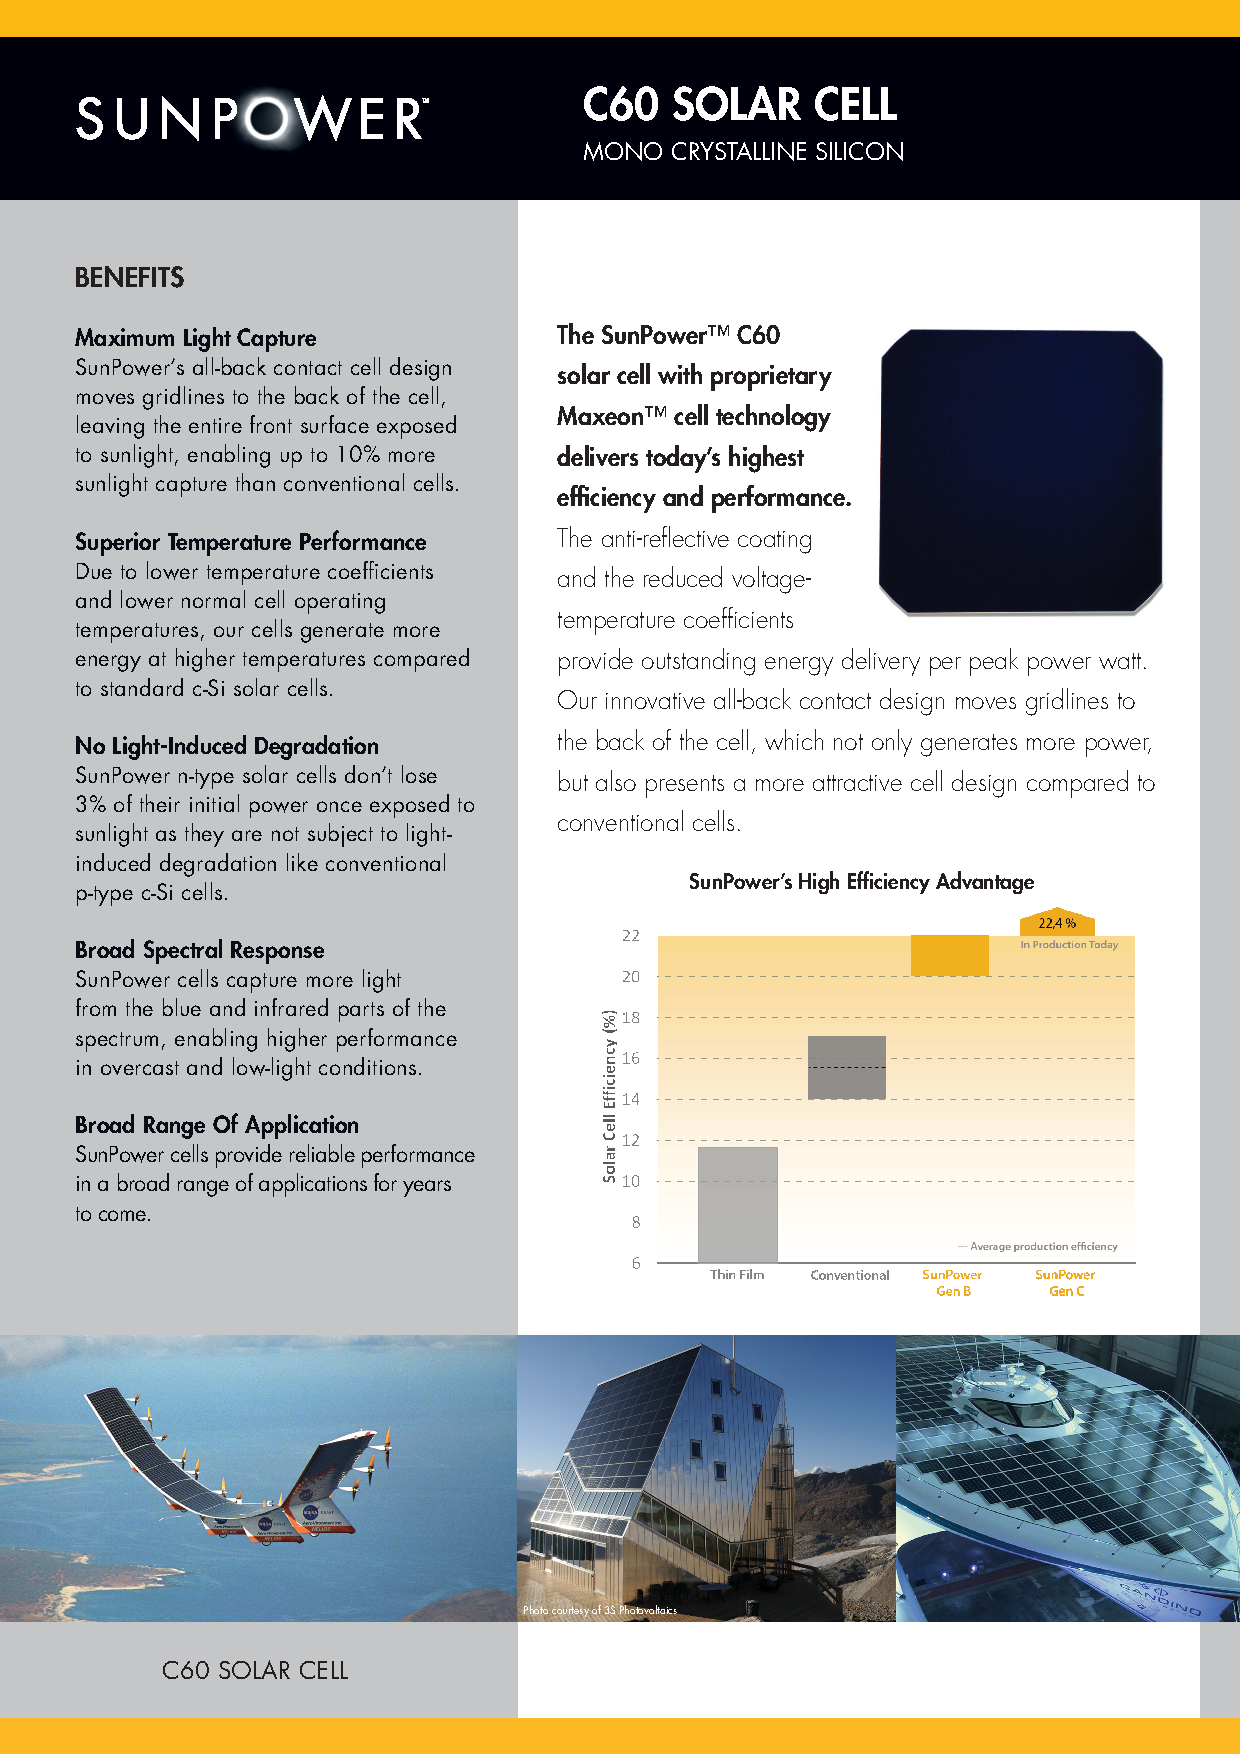
\includepdf[pages={1-2},nup=1x2,landscape=true]{Figures/SolarCell_Sunpower_C60.pdf}

 % file "Thesis_Appendix_B.tex"
%\cleardoublepage

% ----------------------------------------------------------------------
\end{document}
% ----------------------------------------------------------------------

